 
% SET DOCUMENT CLASS, PAGE SETTINGS, FONT...
\documentclass[12pt,a4paper,twoside,openright,justified]{book}

% SET FONT TYPE
\usepackage[T1]{fontenc}
\usepackage{lmodern}
% OTHER FONTS....
%\usepackage{tgpagella}
%\usepackage{mathpazo}

% LOAD PACKAGES...
\usepackage{comment}
\usepackage{appendix}
\usepackage{afterpage}
\newcommand\blankpage{%
    \null
    \thispagestyle{empty}%
    \addtocounter{page}{-1}%
    \newpage}

\usepackage[english,italian]{babel}

\usepackage{csquotes}

\usepackage{hyphenat}

\usepackage{bookabstract}

% SET PAGE MARGINS
\usepackage[top=30mm, bottom=30mm, inner=20mm, outer=20mm, headsep=10mm, footskip=12mm]{geometry}

\usepackage{setspace}
\setstretch{1.4}


\usepackage{lipsum}

\addtolength{\headheight}{3pt}
\usepackage{fancyhdr}
\pagestyle{fancy}% <- must be used before the redefinition of \chaptermark and \sectionmark
% change the marks set by \chapter and \section
\renewcommand{\chaptermark}[1]{\markboth{#1}{}}
\renewcommand{\sectionmark}[1]{\markright{\thesection\ #1}}
% change fancy style
\fancyhf{}
\fancyhead[LE]{\nouppercase{\leftmark}}
\fancyhead[RO]{\nouppercase{\rightmark}}
\fancyfoot[LE,RO]{\thepage}
\renewcommand{\headrulewidth}{0.2pt}

% change plain style (eg. used on chapter pages)
\fancypagestyle{plain}{%
  \fancyhf{}
  \fancyfoot[LE,RO]{\thepage}
  \renewcommand{\headrulewidth}{0pt} % comment this line, if there should be a headsepline on plain pages too
}

% PAGESTYLE IN TOC, LOT, LOF
\fancypagestyle{toclof}{%
  \fancyhf{}%
  \fancyhead[LE]{\nouppercase{\leftmark}}
\fancyhead[RO]{\nouppercase{\rightmark}}
\renewcommand{\headrulewidth}{0.2pt}
  \fancyfoot[LE,RO]{\thepage}
}

% PAGES BETWEEN CHAPTER ARE CLEARED (WHEN LEFTSIDE)
\makeatletter
\renewcommand*{\cleardoublepage}{\clearpage\if@twoside \ifodd\c@page\else
\hbox{}%
\thispagestyle{empty}%
\newpage%
\if@twocolumn\hbox{}\newpage\fi\fi\fi}
\makeatother


% BIBLIOGRAPHY STYLE 
\usepackage[
    backend=biber,
    style=ieee,
    sorting=none,
  ]{biblatex}
\addbibresource{bibliography.bib}

% MANAGE LONG BIBLIOGRAPHY URL
\setcounter{biburlnumpenalty}{9000}
\setcounter{biburlucpenalty}{9000}
\setcounter{biburllcpenalty}{9000}


% SET CHAPTER APPEARENCE (ADD NUMBER NEXT TO THE CHAPTER, MARGIN...)
\usepackage{titlesec}
\titleformat{\chapter}[hang]{\LARGE\bfseries}{\thechapter{. }}{0pt}{\LARGE\bfseries}
\titlespacing*{\chapter}{0pt}{0pt}{15pt} 
\titlespacing*{\section}{0pt}{5pt}{10pt} 
\titlespacing*{\subsection}{0pt}{0pt}{5pt} 
\usepackage{graphicx}

% --- Mathematics ---
\usepackage{bm}         % Bold text in math mode
\usepackage{amsmath}
\usepackage{mathtools}
% SET SPACE ABOVE AND BELOW EQUATION ENVIRONMENT
\makeatletter
\g@addto@macro\normalsize{%
  \setlength\abovedisplayskip{8mm}
  \setlength\belowdisplayskip{8mm}
  \setlength\abovedisplayshortskip{6mm}
  \setlength\belowdisplayshortskip{6mm}
}
\makeatother
% Math formulas and improved typographical quality of their output
\usepackage{amssymb}    % Extended symbol collection
\usepackage{amsthm}     % Helps define theorem-like structures
\usepackage{textcomp}   % Used in the package "gensymb" (below), which will give warnings if "textcomp" is not imported in advance
\usepackage{gensymb}    % Adds extra generic symbols for math and text mode, e.g. \degree

\usepackage{siunitx}
\sisetup{exponent-product=\ensuremath{{}\cdot{}}}

% --- Images caption ---
\usepackage[font=small, labelfont=bf, margin=0.3cm]{caption}        % Enables controlling the look and feel of captions, see package documentation
%\usepackage{subcaption}     % Recommended when making sub-figures
\usepackage[notlof, notlot, nottoc]{tocbibind}  % Includes Bibliography, Index, list of Listing etc. to table of contents
\newcommand{\source}[1]{\vspace{-4pt} \caption*{\hfill \footnotesize{Source: {#1}} } }   % Easily insert sources in images

\usepackage{chngcntr}
\counterwithout{figure}{chapter}
\counterwithout{table}{chapter}
\usepackage{chemformula} % chem formula
\usepackage{chemfig} % chemical fig

\usepackage{booktabs}
\renewcommand{\arraystretch}{1.25} % TABLE LINE SPACING

\usepackage{threeparttable}
\usepackage{threeparttablex}
\usepackage{longtable}
\usepackage{tabularx}
\usepackage{tabularray}
\usepackage{array}
\usepackage[document]{ragged2e}
\usepackage{changepage} 
\usepackage{seqsplit}

\usepackage[version=4]{mhchem}

\usepackage{adjustbox}

\usepackage{subfigure}
\usepackage[subfigure]{tocloft}
\renewcommand{\cftfigpresnum}{\figurename~}
\addtolength{\cftfignumwidth}{13mm}
\renewcommand{\cfttabpresnum}{\tablename~}
\addtolength{\cfttabnumwidth}{13mm}
\setlength{\cftbeforetoctitleskip}{1cm}
\setlength\cftbeforeloftitleskip{1cm}
\setlength\cftbeforelottitleskip{1cm}

\usepackage{lscape}

\usepackage{colortbl}

\usepackage[pdfpagelabels=true]{hyperref}
\hypersetup{
pdftitle={Thesis title},
pdfsubject={Master's degree course},
pdfauthor={Author name},
pdfkeywords={keyword1, keyword2, keyword3}
}

\usepackage{xcolor}
\definecolor{blulink}{HTML}{0F4ACD}
\definecolor{redcite}{HTML}{E34D51}
\hypersetup{
    colorlinks,
    linkcolor={black}, % CHANGE COLOR IF NEEDED
    citecolor={black}, % CHANGE COLOR IF NEEDED
    urlcolor={black}  % CHANGE COLOR IF NEEDED
}

\usepackage[parfill]{parskip}
\setlength\parskip{.5\baselineskip plus .1\baselineskip minus .1\baselineskip}

% SET MAXIMUM DEPTH OF TOC AND SECTIONS
\setcounter{secnumdepth}{4}
\setcounter{tocdepth}{4}

% START THE DOCUMENT
\begin{document}

% INSERT FRONTPAGE
\pagestyle{empty}
% FRONTPAGE SETTINGS (INDEPENDENT GEOMETRY)
\newgeometry{top=25mm,bottom=25mm,inner=25mm,outer=25mm}
\begin{titlepage}

\begin{center}
\thispdfpagelabel{Frontespizio}
{\scshape \Large
University of Modena and Reggio Emilia\\
}
\vspace{5mm}
{\Large
Department of Engineering Enzo Ferrari
}

\rule{145mm}{0.1mm}

\vspace{6mm}
\begin{spacing}{1.8}
{\large\textbf{
Master's Degree Course in\\
}}
{\large\textbf{
Computer Engineering
}}
\end{spacing}
\vspace{30mm}

\begin{spacing}{2.0}
{\Large \bf  Experimental Analysis of Graph RAG}\\
\end{spacing}

\end{center}


\vspace{32mm}
\noindent
\begin{minipage}[t]{0.5\textwidth}
\large
\textbf{Thesis supervisor:
}\\
Prof. Giovanni Simonini\\
 \vspace{5mm}

\end{minipage}
\hfill
\begin{minipage}[t]{0.5\textwidth}\raggedleft
\large
\textbf{Candidate:}\\
Bilel Arfaoui\\

\end{minipage}

\vfill

\begin{center}
\large Academic Year 2023/2024
\end{center}



\end{titlepage}
\restoregeometry


% START QUOTE PAGE
\cleardoublepage
{
\vspace*{0.2\textheight}
\large
\noindent\hfill\enquote{\itshape 
No.
{}}
\bigbreak
}
\large
\hfill Hamlet, Act III, Scene III, Line 87
\normalsize
% END QUOTE PAGE


% SET TEXT STYLE TO JUSTIFIED
\justifying

% SET SPACE BETWEEN TEXT AND FOOTNOTES
\setlength{\skip\footins}{8mm}

% SET PARAGRAPH INDENT
\setlength{\parindent}{0pt}
\setlength{\parskip}{2mm}


% -------------------

% ABSTRACT ENG
\selectlanguage{english}

\begin{abstract}
\thispdfpagelabel{Abstract}

This thesis explores Vector Database Management Systems (VDBMS) as a solution for handling unstructured data by representing them as vector embeddings. We examine the creation of embeddings, compare sparse and dense vector representations, and analyze state-of-the-art indexing techniques such as HNSW and IVF. Additionally, we discuss Approximate Nearest Neighbors (ANN) search and its role in scalable querying, along with filtering methods to enhance retrieval accuracy.  

Beyond querying, we investigate Multi-Modal search, which integrates multiple data types (text, images, and audio) within a unified vector space. We also explore Retrieval-Augmented Generation (RAG), focusing on optimizing retrieval strategies to improve Large Language Model (LLM) responses. Our final experiment compares different RAG techniques, including knowledge graph integration, to refine retrieved contexts and enhance response reliability.  

By evaluating various VDBMS solutions and retrieval methodologies, this thesis aims to provide insights into the evolving landscape of vector-based data management and its applications in modern AI-driven systems.  
\end{abstract}
\thispdfpagelabel{8}

% SELECT MAIN LANGUAGE (eng or ita), AFTER ENGLISH ABSTRACT AND GRAPHICAL ABSTRACT
\selectlanguage{english}
%\selectlanguage{italian}


% START FRONTMATTER (Table Of Contents, List Of Tables, List Of Figures) - ROMAN NUMERALS
\frontmatter
\begin{spacing}{1.3}
\pagestyle{toclof}
\tableofcontents  % INSERT TABLE OF CONTENTS
\clearpage
%\listoffigures % INSERT LIST OF FIGURES
%\clearpage
%\listoftables % INSERT LIST OF TABLES
%\clearpage
\end{spacing}


% --------------------------
% START THESIS (Arabic numerals)
\mainmatter

% INTRODUCTION
% INTRODUCTION FILE
\pagestyle{fancy}
\chapter*{Introduction}
\pagestyle{fancy}
The exponential growth of unstructured data, such as text, images, and audio, has outpaced the capabilities of traditional relational databases, which are optimized for structured records and ACID compliance. While conventional databases excel at transactional consistency, they struggle with efficient retrieval and similarity search across high-dimensional data spaces. This challenge has led to the rise of \textbf{Vector Database Management Systems (VDBMS)}, which represent data as vector embeddings, enabling powerful search and retrieval mechanisms based on similarity rather than exact matching.  

VDBMS leverage Approximate Nearest Neighbors (ANN) search to efficiently query large-scale datasets, balancing speed and accuracy. Unlike traditional indexing methods, vector databases employ structures such as \textbf{Hierarchical Navigable Small World (HNSW) graphs} and \textbf{Inverted File Index (IVF)} to optimize search performance. Additionally, quantization techniques reduce memory and storage footprints while preserving retrieval quality.  

Beyond retrieval, the application of VDBMS extends to \textbf{Multi-Modal search}, where different data types—such as images, text, and audio—are mapped into a unified vector space for seamless cross-modal querying. Furthermore, the integration of VDBMS with \textbf{Retrieval-Augmented Generation (RAG)} has gained traction, enhancing Large Language Model (LLM) responses by retrieving relevant context from vectorized data sources.  

This thesis explores the architecture, indexing techniques, and retrieval strategies of modern VDBMS. It evaluates leading implementations such as Weaviate, FAISS, and Milvus, comparing their performance in large-scale search applications. Additionally, we investigate the role of vector databases in \textbf{Agentic RAG}, examining strategies to mitigate issues improve retrieval precision through knowledge graphs and optimized prompting techniques.  

This work explores the capabilities and limitations of Vector Database Management Systems (VDBMS) to provide a comprehensive understanding of their impact on AI-driven search and retrieval. We highlight their role as a foundational technology in modern information systems. Finally, we introduce and analyze GraphRAG, a novel retrieval technique, comparing it to vector-based RAG. We examine their respective applications, advantages, and limitations, illustrating different use cases. As a final experiment, we propose an architecture for join discovery, leveraging knowledge graphs as a knowledge base to link entities and tables, enabling users to query structured data using natural language prompts.


% CHAPTER 1
\pagestyle{fancy}
\chapter{Vector Representation of Data}
\label{chap:first_chapter}

In this chapter, we will explore the field of unstructured data, discussing how it differs from the traditional structured approach and how it plays a crucial role in modern applications. We will examine the process of converting unstructured data into vectorized representation and what it entails. Additionally we will introduce Vector Database Management Systems, exploring their architecture, functionalities and their impact on the market.

\section{Unstructured Data vs. Structured Data}
In the context of data management, data can be classified as structured or unstructured. Structured data refers to information arranged in rows and columns, typically found in relational databases. These follow a defined schema and are used to store records or transactions within a database environment. Meanwhile, unstructured data lack predefined formats and cannot be easily arranged into columns. Examples include text, audio, images, documents, and videos. This characteristic makes efficient indexing, organization, and retrieval challenging.
\begin{figure}[h]
    \centering
    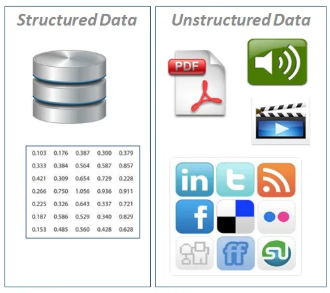
\includegraphics[width=0.4\textwidth]{IMAGES/immagine_2025-02-24_091828425.png}
    \label{fig:Structured vs. Unstructured data}
    \caption[Structured vs. Unstructured data.]{Structured vs. Unstructured data. Source: DeepLearning.AI. \footnotemark.}
    \label{fig:structuredVunstruct}
\end{figure}
\footnotetext{\url{https://www.deeplearning.ai/short-courses/building-multimodal-search-and-rag/}}

Today’s digital services and applications generate vast amounts of data, whose scale suggests that valuable insights can be extracted. If organized effectively, such data can significantly aid stakeholders in long-term decision-making processes.

\section{From Raw Data to Vector Representation}
A vector embedding is a numerical representation of data (such as images, documents, and audio) that encapsulates meaning, characteristics, and associations. This representation enables unstructured data to be interpreted by computational systems, unlocking numerous use cases and applications. The embedding process maps objects and entities into a vector space, where dimensionality is determined by the encoding model.

\begin{figure}[h]
    \centering
    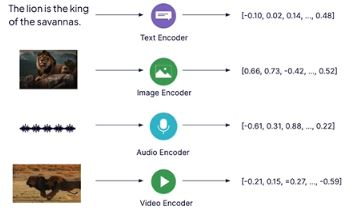
\includegraphics[width=0.5\textwidth]{IMAGES/encode.JPG}
    \caption[Encoding process.]{Encoding process. Source: DeepLearning.AI.\footnotemark.}
    \label{fig:Encoding}
\end{figure}

\footnotetext{\url{https://www.deeplearning.ai/short-courses/building-multimodal-search-and-rag/}}

Thanks to this structure, machine learning techniques can analyze unstructured data, uncover patterns, and generate insights. These techniques are widely applied in fields such as Natural Language Processing (NLP), Computer Vision, Recommendation Systems, and Search Engines. Each application comes with its own challenges. Another key advantage of mathematical vector representations is their ability to facilitate computational efficiency and scalability in data processing.
\section{Dense vs. Sparse Vectors}

It is important to distinguish between two types of vector embeddings: dense and sparse. Dense embeddings have lower dimensionality, with each value carrying meaningful information, while sparse embeddings have high dimensionality but contain only a few non-zero values. Typically, dense vectors are obtained through deep learning techniques or by applying dimensionality reduction to sparse vectors. Each representation has its own strengths, limitations, and use cases, and they can also be effectively combined in certain applications.

\subsubsection{Sparse Vectors}

Sparse embeddings are commonly used in NLP and recommender systems, where data often has high dimensionality but each instance activates only a few features. In a typical sparse vector, each dimension represents a token, and the value indicates that token’s importance within a document. This makes sparse vectors particularly advantageous for applications requiring keyword matching. Several methods exist for creating sparse vectors:

\begin{itemize}
    \item \textbf{Bag of Words (BOW)}: Simple and interpretable, but ignores word order and context.
    \item \textbf{One-Hot Encoding}: Clearly maps each token but results in extremely high dimensionality with large vocabularies.
    \item \textbf{TF-IDF}: Highlights unique terms and relevance within a document but does not capture semantic relationships.
    \item \textbf{BM25}: Extends TF-IDF by considering term frequency and document length but requires full corpus statistics in advance.
    \item \textbf{Sparse Neural Embeddings}: Uses neural networks for efficient keyword matching on large datasets, though often less interpretable than traditional methods.
\end{itemize}

However, sparse vectors struggle to capture nuanced relationships between words. Each dimension may correspond to a word or subword grouping, which aids in interpreting document rankings. Sparse vectors are particularly useful in scenarios with rare keywords or specialized terms that may not appear in standard vocabularies, where general-purpose embeddings might fail to convey the intended meaning. They are highly effective for text search and hybrid search applications.

\subsubsection{Dense Vectors}

Dense embeddings are widely used in NLP and machine learning to capture complex relationships within data. Unlike sparse vectors, dense embeddings represent rich, context-sensitive information in lower-dimensional space, making them ideal for tasks such as semantic search and sentence similarity. While they excel at capturing nuanced meanings, dense embeddings can be computationally intensive and less interpretable. Deep learning techniques are typically used to generate these embeddings, learning from large datasets to uncover intricate patterns. In many cases, dense and sparse vectors can be combined to take advantage of both.

\section{Vector Database Architecture}  

Vector databases share several core components that enable efficient storage, retrieval, and querying of vector embeddings:  

\begin{itemize}  
    \item \textbf{Client Interface}: Provides API or GUI access for querying and managing data.  
    \item \textbf{Query Processor}: Handles similarity searches using distance metrics and ranking mechanisms.  
    \item \textbf{Vector Storage}: Stores vector embeddings and associated metadata.  
    \item \textbf{Indexing Module}: Manages indexing structures to enable efficient retrieval.  
    \item \textbf{Embedding Generation Module}: Converts raw unstructured data (e.g., text, images, audio) into high-dimensional vector embeddings using traditional or deep learning techniques.  
\end{itemize}  
\begin{figure}[h]
    \centering
    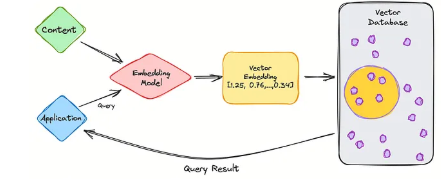
\includegraphics[width=0.6\textwidth]{IMAGES/immagine_2025-02-24_100130378.png}
    \caption[VDB Architecture.]{Architecture. Source: Medium.\footnotemark.}
    \label{fig:Architecture}
\end{figure}
\footnotetext{\url{https://medium.com/data-and-beyond/vector-databases-a-beginners-guide-b050cbbe9ca0}}
\subsection{Querying and Search Efficiency}  
Vector databases balance speed and accuracy using Approximate Nearest Neighbor (ANN) search techniques. These approaches enable efficient retrieval without performing exhaustive comparisons, making them well-suited for large-scale datasets.  

\subsection{Scalability Considerations}  
Handling high-dimensional data efficiently requires scalable solutions. VectorDBs achieve scalability through distributed architectures, memory-efficient indexing, and cloud-based deployments. These capabilities make them viable for both on-premise and large-scale cloud environments.  








\section{Multimodal Vector Space}
One key application of vector DBMSs is the mapping of data in Multimodal Vector Spaces, which refers to the storage and retrieval of data across multiple modalities, such as text, images, audio and video, in a unified embedding space. This means that conceptually related items, regardless of their format (e.g., an image of a lion and the phrase "the king of the jungle"), are placed close to each other in this space.
\begin{figure}[h]
    \centering
    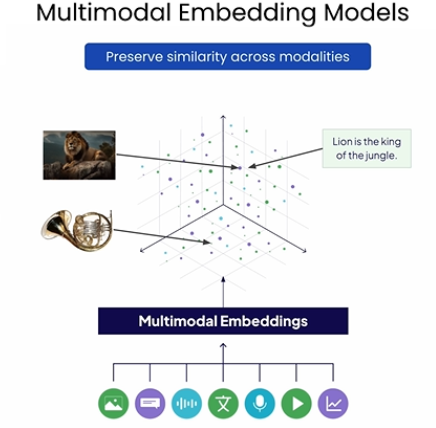
\includegraphics[width=0.5\textwidth]{IMAGES/immagine_2025-02-23_214815401.png}
    \caption{Multimodal Vector Space.}
    \label{fig:multimodal_space}
    \source{\url{https://www.deeplearning.ai/short-courses/building-multimodal-search-and-rag/}}
\end{figure}

The key motivation for multimodal data comes from the fact that humans understand the world, not through a single mode like text alone, but through a combination of sensory inputs. For example, hearing the sound of a cash register can immediately evoke the concept of a store or a purchase. By integrating multiple modalities, we aim to develop systems capable of learning and reasoning across diverse data formats. 
\subsection{Constructing the Multimodal Vector Space}
To achieve this, we employ specialized encoders that learn representations for each modality separately and then align them through contrastive learning.
The process of constructing a Multimodal vector space consists of the following steps:
\begin{enumerate}
    \item Train individual embedding models for each modality (e.g., an image encoder for images, a text encoder for text).
    \item Align these models in a shared vector space.
    \item Optimize the embeddings to ensure cross-modal similarity.
    \item Use contrastive learning to fine-tune the models by distinguishing between positive and negative examples.
\end{enumerate}
\subsection{Applications of Multimodal Retrieval}
Multimodal retrieval has various real-world applications, including:
\begin{itemize}
    \item \textbf{Image-Text Search}: Finding relevant images based on textual queries (e.g., retrieving an image of the Eiffel Tower when searching "Paris landmark").
    \item \textbf{Video Retrieval}: Searching for specific moments in videos using natural language queries.
    \item \textbf{Audio-Visual Understanding}: Associating spoken words with corresponding visual elements in video content.
    \item \textbf{Medical Imaging}: Aligning radiology reports with corresponding X-ray images to enhance diagnostics.
\end{itemize}



\section{Key Products and Features}
The following are leading vector database solutions available in the market:
\begin{itemize}
    \item \textbf{Milvus:} Open-source, distributed database optimized for scalability and GPU acceleration, widely used in AI analytics and recommendation systems.
    \item \textbf{Pinecone:} Managed service with real-time indexing, automatic scaling, and seamless ML integration, ideal for semantic search and anomaly detection.
    \item \textbf{QDrant:} High-performance, open-source vector search engine supporting hybrid search (vector + metadata), multimodality and efficient memory management.
    \item \textbf{Weaviate:} Similar to QDrant offering flexible filtering and retrieval strategies.
\end{itemize}

\chapter{Vectorization Techniques}
In this chapter, we will explore vectorization techniques in depth, beginning with traditional methods such as One-Hot Encoding, Bag of Words, and TF-IDF. We will then transition into fundamental Deep Learning principles, which lay the groundwork for advanced representations, including word embeddings and transformer-based models, enabling richer, context-aware representations. Furthermore Deep Learning principles will serve as context for advanced applications of Vector Databases in the following chapters.

\section{Traditional Vectorization Techniques}
Traditional vectorization techniques transform textual data into numerical representations, enabling computational processing and analysis. These methods primarily rely on statistical properties of text rather than learned representations from deep learning models. This section explores widely used traditional techniques, including One-Hot Encoding (OHE), Bag of Words (BoW), Term Frequency-Inverse Document Frequency (TF-IDF).

\subsection{Tokenization}  
Tokenization is a crucial preprocessing step for both traditional and deep learning-based vectorization. It involves breaking text into smaller units (tokens), with different approaches offering various trade-offs:  

\begin{itemize}  
    \item \textbf{Byte-level tokenization}: Operates on a small vocabulary, encoding text at the byte level.  
    \item \textbf{Word-based tokenization}: Uses full words as tokens, preserving meaning but struggling with unseen words due to a large vocabulary.  
    \item \textbf{Subword tokenization}: A compromise between the two, capturing word roots (e.g., NLP, lemmatization) while remaining trainable and statistically driven.  
\end{itemize}  



\subsection{One-Hot Encoding (OHE)}

One-Hot Encoding (OHE) is the simplest vectorization technique, representing each unique word in a vocabulary as a binary vector. Given a vocabulary of size \( V \), each word \( w_i \) is mapped to a vector of length \( V \) where only the corresponding index is set to 1, while all other elements remain 0. 

For example, given the vocabulary:
\[
\{ \text{apple}, \text{banana}, \text{cherry} \}
\]
the one-hot encoded vectors are:

\[
\text{apple} \rightarrow [1, 0, 0], \quad
\text{banana} \rightarrow [0, 1, 0], \quad
\text{cherry} \rightarrow [0, 0, 1]
\]

Mathematically, for a given word \( w_i \) in a vocabulary of size \( V \), its one-hot representation \( \mathbf{v}_{w_i} \) is:

\begin{equation}
    \mathbf{v}_{w_i} = [0, 0, \dots, 1, \dots, 0, 0]
\end{equation}

where the position of 1 corresponds to the index of the word in the vocabulary.

While simple and interpretable, one-hot encoding suffers from high dimensionality and sparsity, making it inefficient for large vocabularies. Additionally, it does not capture semantic relationships between words (e.g., "cat" and "dog" are equally distant from "fish" in this representation).

\subsection{Bag of Words (BoW)}

The Bag of Words model extends OHE by considering word frequencies in a document rather than binary presence. It represents a document by counting the occurrences of words, ignoring word order and syntax. Formally, let \( D \) be a collection of documents and \( V \) the vocabulary of unique words across all documents. The BoW representation of a document \( d \) is a vector:

\begin{equation}
    \mathbf{v}_d = (f_1, f_2, \dots, f_n)
\end{equation}

where \( f_i \) is the frequency of word \( w_i \) in the document \( d \). While BoW is effective in some applications, it suffers from high dimensionality and lacks semantic understanding.

\subsection{Term Frequency-Inverse Document Frequency (TF-IDF)}

TF-IDF improves upon the BoW model by assigning importance to words based on their frequency across multiple documents. The TF-IDF value for a word \( w \) in a document \( d \) is given by:

\begin{equation}
    \text{TF-IDF}(w, d) = \text{TF}(w, d) \times \text{IDF}(w)
\end{equation}

where:
\begin{itemize}
    \item \textbf{Term Frequency (TF)} measures how frequently a word appears in a document:
    \begin{equation}
        \text{TF}(w, d) = \frac{f_w}{\sum_{w' \in d} f_{w'}}
    \end{equation}
    where \( f_w \) is the count of word \( w \) in document \( d \).

    \item \textbf{Inverse Document Frequency (IDF)} reduces the weight of common words appearing in many documents:
    \begin{equation}
        \text{IDF}(w) = \log \left( \frac{N}{1 + \text{DF}(w)} \right)
    \end{equation}
    where \( N \) is the total number of documents, and \( \text{DF}(w) \) is the number of documents containing \( w \).
\end{itemize}

TF-IDF effectively emphasizes informative words while downplaying common ones, making it useful for tasks like document classification and search retrieval.

\section{Deep Learning}
The conversion of unstructured data to vector embedding is an automatic process that leverages Deep Learning techniques by using Neural Networks, which is essentially a computational model inspired by how the human brain processes information, in a nutshell Neural Networks are composed of layers of interconnected “neurons” that perform calculations on the input data.

\subsection{Neuron}
The “Neuron” is the most basic computational unit of the Neural Network, each neuron takes multiple inputs, each with an associated weight (which indicates the importance), computes their weighted sum, adds a constant called bias, and then passes this result through an activation function, which generates the neuron's output.
\begin{figure}[h]
    \centering
    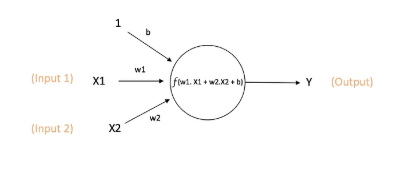
\includegraphics[width=0.6\textwidth]{IMAGES/immagine_2025-02-26_153339240.png}
    \caption[Neuron]{Neuron Source.\footnotemark.}
    \label{fig:Neuron}
\end{figure}
\footnotetext{\url{https://medium.com/analytics-vidhya/neural-networks-in-a-nutshell-bb013f40197d}}

The most popular and widely known activation functions in neural networks are:
\begin{itemize}
    \item \textbf{Sigmoid}: \( \sigma(x) = \frac{1}{1 + e^{-x}} \)
    \item \textbf{Tanh}: \( \tanh(x) = \frac{e^x - e^{-x}}{e^x + e^{-x}} \)
    \item \textbf{ReLU}: \( f(x) = \max(0, x) \)
    \item \textbf{Softmax}: \( \sigma(x_i) = \frac{e^{x_i}}{\sum_{j} e^{x_j}} \)
\end{itemize}

As said before the neural networks is has an architecture that is composed by layers each one with its neurons, they are the following:

\begin{itemize}
    \item \textbf{Input layer}: Which is responsible to receive the input data.
    \item \textbf{Output Layer}: Responsible for producing the final result.
    \item \textbf{Hidden Layer/s}:One or more layers situated between the input and output layers of a neural network, they process and transform the data to help the network learn complex patterns.
\end{itemize}
The number of neurons in each layer and the way they are interconnected depend entirely on the network's design, which is tailored to suit the specific use case.
\subsection{Training process}
Once the neural network architecture is defined, it needs to be trained, which is an iterative process where each iteration called “epoch” is composed of three main steps: Forward propagation, calculation of loss, Backward propagation. The forward propagation starts with initializing the weights and bias (non zero number) and the calculation of the output is done. Then the network's output is compared to the expected result using a loss function. After calculating the loss function, the last step of the iteration is Backward propagation, which through an optimizer adjusts the parameters (weights and biases). The dataset used for training is typically employed in batches, doing so the network trains on each batch on each epoch.


\section{Autoencoders}
One of the architectures used to create vector embeddings leveraging neural networks, is the Autoencoder, a type of neural network with three main parts: encoder layers (which compress the input), a bottleneck layer (where the compact embedding is stored), and decoder layers (which try to rebuild the original input). 
\begin{figure}[h]
    \centering
    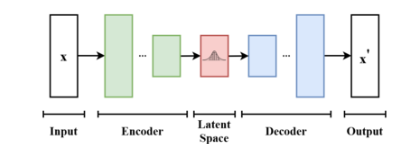
\includegraphics[width=0.6\textwidth]{IMAGES/immagine_2025-02-26_154609390.png}
    \caption[AutoEncoder]{Autoencoder Source.\footnotemark.}
    \label{fig:Autoencoder}
\end{figure}
\footnotetext{\url{https://www.deeplearning.ai/short-courses/building-multimodal-search-and-rag/}}
Basically the encoder layers gradually reduce the number of neurons, compressing the data until it reaches the bottleneck layer. The decoder layers then expand the data again to reconstruct the original input. The vector embedding of the raw data corresponds to the output of the bottleneck layer, and its dimensionality is determined by the number of neurons in that layer. Since the network compresses and decompresses the data, some information is lost in the process, but with proper training the weights will be adjusted to minimize the loss. 
\subsection{Example with the MINST dataset}
As an example, we use the MNIST dataset, which consists of images of handwritten digits. The neural network architecture, shown in the figure below, is an autoencoder with two layers in both the encoder and decoder. The encoder progressively compresses the data from 256 dimensions to 128 and then to 2 dimensions in the bottleneck layer, while the decoder reverses this process to reconstruct the original input. The network uses dense layers, meaning each neuron is fully connected to the neurons in the following layer.
\begin{figure}[h]
    \centering
    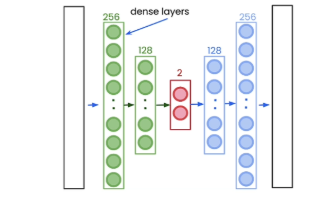
\includegraphics[width=0.6\textwidth]{IMAGES/immagine_2025-02-26_154914801.png}
    \caption[Example of AutoEncoder]{example of AutoEncoder dimensions:
 Source.\footnotemark[3]}
    \label{fig:2D}
\end{figure}
\footnotetext[3]{\url{https://www.deeplearning.ai/short-courses/building-multimodal-search-and-rag/}}

For simplicity and clarity, the images are represented as 2-dimensional vectors, as shown in the plot below.

\begin{figure}[h]
    \centering
    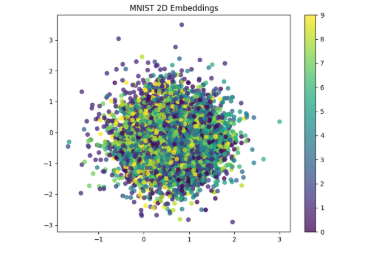
\includegraphics[width=0.6\textwidth]{IMAGES/immagine_2025-02-26_155006209.png}
    \caption[MNIST 2D]{MNIST mapped in 2D:
 Source.\footnotemark[3]}
    \label{fig:2D}
\end{figure}


As expected, some information is lost during the compression process, as the input and output images are not identical. However, by adjusting the weights, the network can minimize this loss and produce outputs closer to the original.
\begin{figure}[h]
    \centering
    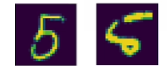
\includegraphics[width=0.6\textwidth]{IMAGES/immagine_2025-02-26_155109338.png}
    \caption[MNIST Results]{Before and After encoding:
 Source.\footnotemark[3]}
    \label{fig:2D}
\end{figure}

In the context of VectorDBs, the encoder is the more relevant component, as it outputs the embeddings needed for database operations. Embeddings can be produced by pre-trained or use-case specific models in order to capture insights.
As shown above, it’s easy for a person to recognize that the first two images represent the same entity. Thanks to the mathematical properties of embeddings, we can make this relationship machine-understandable. By using a similarity function, the system can also determine which pairs of images are more similar
\section{Evolution to Context aware techniques}
While autoencoders provide a compressed representation of the data, and can be trained in an unsupervised way, they still require a training dataset and do not capture contextual relationships. For these reasons, next step mechanisms of that capture the contextual dependencies have been developed such as Recurrent Neural Networks (RNNs) and Long Short-Term Memory Networks (LSTMs), which we will briefly show their functionalities and how they paved the way to Transformers.

\subsection{Recurrent Neural Networks (RNNs)}

Recurrent Neural Networks (RNNs) introduced the idea of modeling sequential dependencies by maintaining a hidden state \( h_t \) that evolves over time:

\begin{equation}
    h_t = f(W_h h_{t-1} + W_x x_t + b),
\end{equation}

where \( W_h \) and \( W_x \) are weight matrices, \( b \) is a bias term, and \( f \) is an activation function (e.g., tanh or ReLU). However, RNNs suffer from the \textit{vanishing gradient problem}, meaning that the gradient the derivative of the loss function, which provides information information of the direction that the model is taking, becomes very small during backpropagation, making it difficult to learn long-range dependencies.
\subsection{LSTM}
LSTMs (Long Short-Term Memory networks) improve upon standard RNNs (Recurrent Neural Networks) by introducing a \textbf{memory cell} \( C_t \) and \textbf{gating mechanisms} that control the flow of information over time. This allows the network to "remember" important information for longer periods and "forget" irrelevant data.
At each time step \( t \), the LSTM takes the input \( x_t \) and the previous hidden state \( h_{t-1} \), and updates the memory cell \( C_t \) and hidden state \( h_t \). The LSTM consists of the following components:

\begin{itemize}
    \item The \textbf{forget gate} \( f_t \) decides how much of the previous memory \( C_{t-1} \) should be kept.
    \item The \textbf{input gate} \( i_t \) controls how much new information \( \tilde{C}_t \) should be added to the memory cell.
    \item The \textbf{output gate} \( o_t \) decides what part of the memory cell \( C_t \) should be output as the current hidden state \( h_t \).
\end{itemize}

The memory cell is updated as follows:

\[
C_t = f_t \odot C_{t-1} + i_t \odot \tilde{C}_t
\]

where \( \tilde{C}_t \) is the candidate memory, computed from the input \( x_t \) and previous hidden state \( h_{t-1} \). The hidden state is then computed as:

\[
h_t = o_t \odot \tanh(C_t)
\]
\subsection{The Transformer Architecture}
Transformers address LSTMs' scalability issues by processing entire sequences simultaneously using self-attention, the core mechanism of the architecture. Self-attention allows the model to interpret a word’s meaning based on its context, even when the same word has different meanings. The self-attention mechanism computes attention scores as:
\begin{equation}
A = \frac{QK^T}{\sqrt{d_k}}
\end{equation}
where  are the query, key, and value matrices derived from input embeddings. Specifically:
\begin{itemize}
\item  \textbf{Q}(Query): Represents the current word/token for which attention is being computed.
\item  \textbf{K}(Key): Represents all words/tokens in the sequence, determining relevance.
\item  \textbf{V}(Value): Contains the actual token representations used to construct the final weighted output.
\end{itemize}
These matrices are obtained by linearly transforming the input embeddings using learned weight matrices :
\begin{equation}
Q = X W_Q, \quad K = X W_K, \quad V = X W_V.
\end{equation}
The attention scores are normalized using softmax and then we compute the final representation with V:
\begin{equation}
    Z = \text{softmax}\left( \frac{QK^T}{\sqrt{d_k}} \right)V.
\end{equation}
Multi-head attention enhances this mechanism by capturing multiple representation aspects, each attention head processes the input independently with learned projections:  
\[
\text{head}_i = \text{Attention}(Q W_i^Q, K W_i^K, V W_i^V),
\]  
where \( W_i^Q \), \( W_i^K \), and \( W_i^V \) are learned projection matrices for queries, keys, and values, respectively. The outputs of all \( h \) heads are concatenated and linearly transformed using another learned weight matrix \( W^O \):  
\[
\text{MultiHead}(Q, K, V) = \text{Concat}(\text{head}_1, \dots, \text{head}_h) W^O.
\]  
Here, \( W^O \) ensures that the final output maintains the desired dimensionality for subsequent layers.
\subsubsection{GPT: Autoregressive Transformer Models}  
The Generative Pre-trained Transformer (GPT) series, along with models like Mistral and LLaMA 2, follows an \textbf{autoregressive} architecture, predicting one token at a time based on prior tokens:  
\begin{equation}
    P(x_t | x_1, x_2, ..., x_{t-1})
\end{equation}  
GPT uses \textbf{causal self-attention}, ensuring tokens only attend to past inputs, making it effective for text generation. It is trained unsupervised on vast text corpora using next-token prediction. During training, a prompt like \textit{"Jack and Jill went over..."} leads the model to assign probabilities to possible next tokens. Training involves guiding initial tokens (e.g., forcing \textit{"The Rock"} for \textit{"The rock at first..."}) and continuing until reaching a token limit or an \texttt{[EOS]} token.  
\begin{figure}[h]
    \centering
    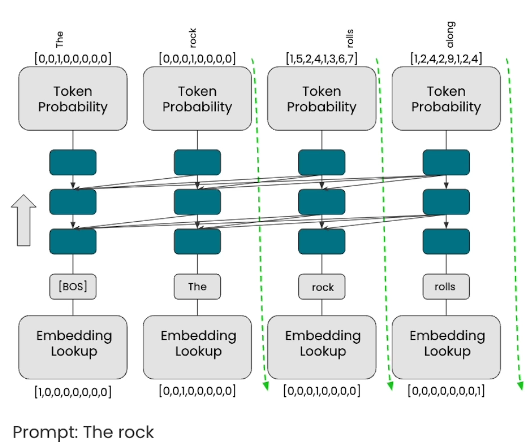
\includegraphics[width=0.4\textwidth]{IMAGES/immagine_2025-02-26_110808787.png}
    \caption[GPT]{GPT model example. Source: DeepLearning.AI.\footnotemark.}
    \label{fig:GPT model}
\end{figure}
\footnotetext{\url{https://www.deeplearning.ai/short-courses/building-multimodal-search-and-rag/}}
\subsection{Visual Transformers (ViTs)}

Visual Transformers extend the principles of self-attention, initially designed for textual data, to computer vision tasks. A Vision Transformer (ViT) processes an image by dividing it into patches, embedding each patch, and applying a transformer model to classify the image based on its patch representations.

\begin{figure}[h]
    \centering
    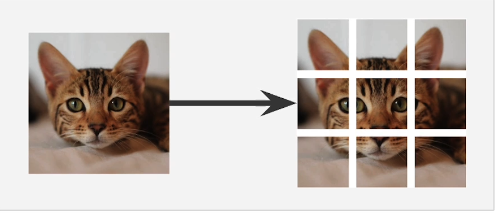
\includegraphics[width=0.4\textwidth]{IMAGES/immagine_2025-02-26_112843716.png}
    \caption[Image Patching]{Image patching. Source: DeepLearning.AI.\footnotemark[4]}
    \label{fig: Patching }
\end{figure}

Key steps in ViT include:

\begin{itemize}
    \item \textbf{Patch Embedding}: An input image of size \( H \times W \) is divided into non-overlapping patches of size \( P \times P \), flattened, and projected into an embedding space.
    \item \textbf{Positional Encoding}: Added to embeddings to retain spatial information.
    \item \textbf{Multi-Head Self-Attention}: Computes relationships across patches.
    \item \textbf{Classification Head}: Uses a CLS token for final classification.
\end{itemize}

\begin{figure}[h]
    \centering
    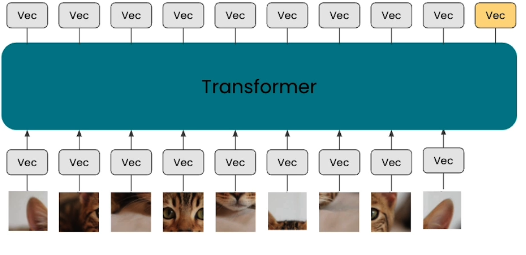
\includegraphics[width=0.4\textwidth]{IMAGES/immagine_2025-02-26_112630864.png}
    \caption[Vision Transformer]{Vision Transformer process. Source: DeepLearning.AI.\footnotemark[4]}
    \label{fig:Vi Transformer }
\end{figure}
\footnotetext[4]{\url{https://www.deeplearning.ai/short-courses/building-multimodal-search-and-rag/}}

\section{Training LLMs to See Images and Multimodality}
Recent advancements in multimodal learning have enabled Large Language Models (LLMs) to not only process text but also understand and generate responses based on visual inputs. One key approach to achieve this is \textbf{Visual Instruction Tuning}. In this process, an LLM is trained to take both visual and textual inputs, allowing it to generate appropriate responses to prompts that involve both types of data. For instance, when given an image of a painting and a prompt like "Who drew this painting?", the model can correctly respond with "Vincent Van Gogh."

\subsection{Multimodal Learning Process}
Large Language Models can be trained to process visual and language input, the process starts with patching and embedding the images as shown before. Moreover, the text prompt is also embedded in a vector space. The model then processes these embeddings, representing both visual and textual information. The core of the model’s training involves integrating these two types of embeddings—\textit{visual embeddings} (from image patches) and \textit{language embeddings} (from text). This allows the model to consider both image and text inputs when generating a response, making it capable of handling Multimodal requests.
\begin{figure}[h]
    \centering
    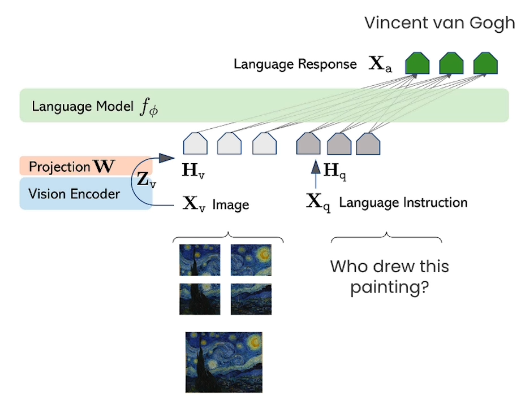
\includegraphics[width=0.6\textwidth]{IMAGES/immagine_2025-02-26_113532424.png}
    \caption[Text and Image input processed]{Text and Image input processed. Source: DeepLearning.AI.\footnotemark[4]}
    \label{fig:InputText}
\end{figure}
The resulting model can handle tasks that require both visual understanding and language generation, such as identifying objects in an image or answering questions about visual content.

\subsection{Large Multimodal Models (LMMs)}
\textbf{Large Multimodal Models (LMMs)} take this integration even further by combining multiple types of data—text, images, audio, and video—into a single model. These models extend the capabilities of traditional LLMs by processing and understanding a wider range of inputs, which enables more sophisticated, context-aware AI systems.

\subsection{Key Components of Multimodal Learning}

Multimodal learning is the process of combining and aligning different types of data to produce richer and more meaningful representations. The main components of LMMs include:

\begin{itemize}
    \item \textbf{Modality-Specific Encoders}: Each modality (e.g., text, image, audio) is processed by a dedicated encoder. For example, in CLIP (Contrastive Language-Image Pretraining), distinct encoders handle the text and image inputs, learning a shared embedding space that links the two modalities.
  
    \item \textbf{Cross-Attention Mechanisms}: These mechanisms allow the model to exchange information between different modalities, enhancing the model's understanding of the data. For example, this helps the model connect visual features with corresponding textual descriptions.
  
    \item \textbf{Unified Representations}: The model fuses the multimodal inputs into a single vector space, facilitating tasks like generation and retrieval that require understanding and synthesizing information across modalities.
\end{itemize}

\subsection{Contrastive Learning for Multimodal Embeddings}
Contrastive learning plays a key role in aligning embeddings from different modalities. The goal is to learn a representation where similar data points (positive pairs) are drawn closer together, while dissimilar ones (negative pairs) are pushed further apart.
\subsubsection{Contrastive Learning Procedure}
The contrastive learning process follows these steps:
\begin{enumerate}
    \item Define an anchor (e.g., an image of a cat).
    \item Identify a positive example, which is semantically related to the anchor (e.g., the phrase "a small feline").
    \item Identify a negative example, which is unrelated to the anchor (e.g., an image of a car).
    \item Train the model to minimize the distance between the anchor and the positive example while maximizing the distance to the negative example.
\end{enumerate}

\begin{figure}[h]
    \centering
    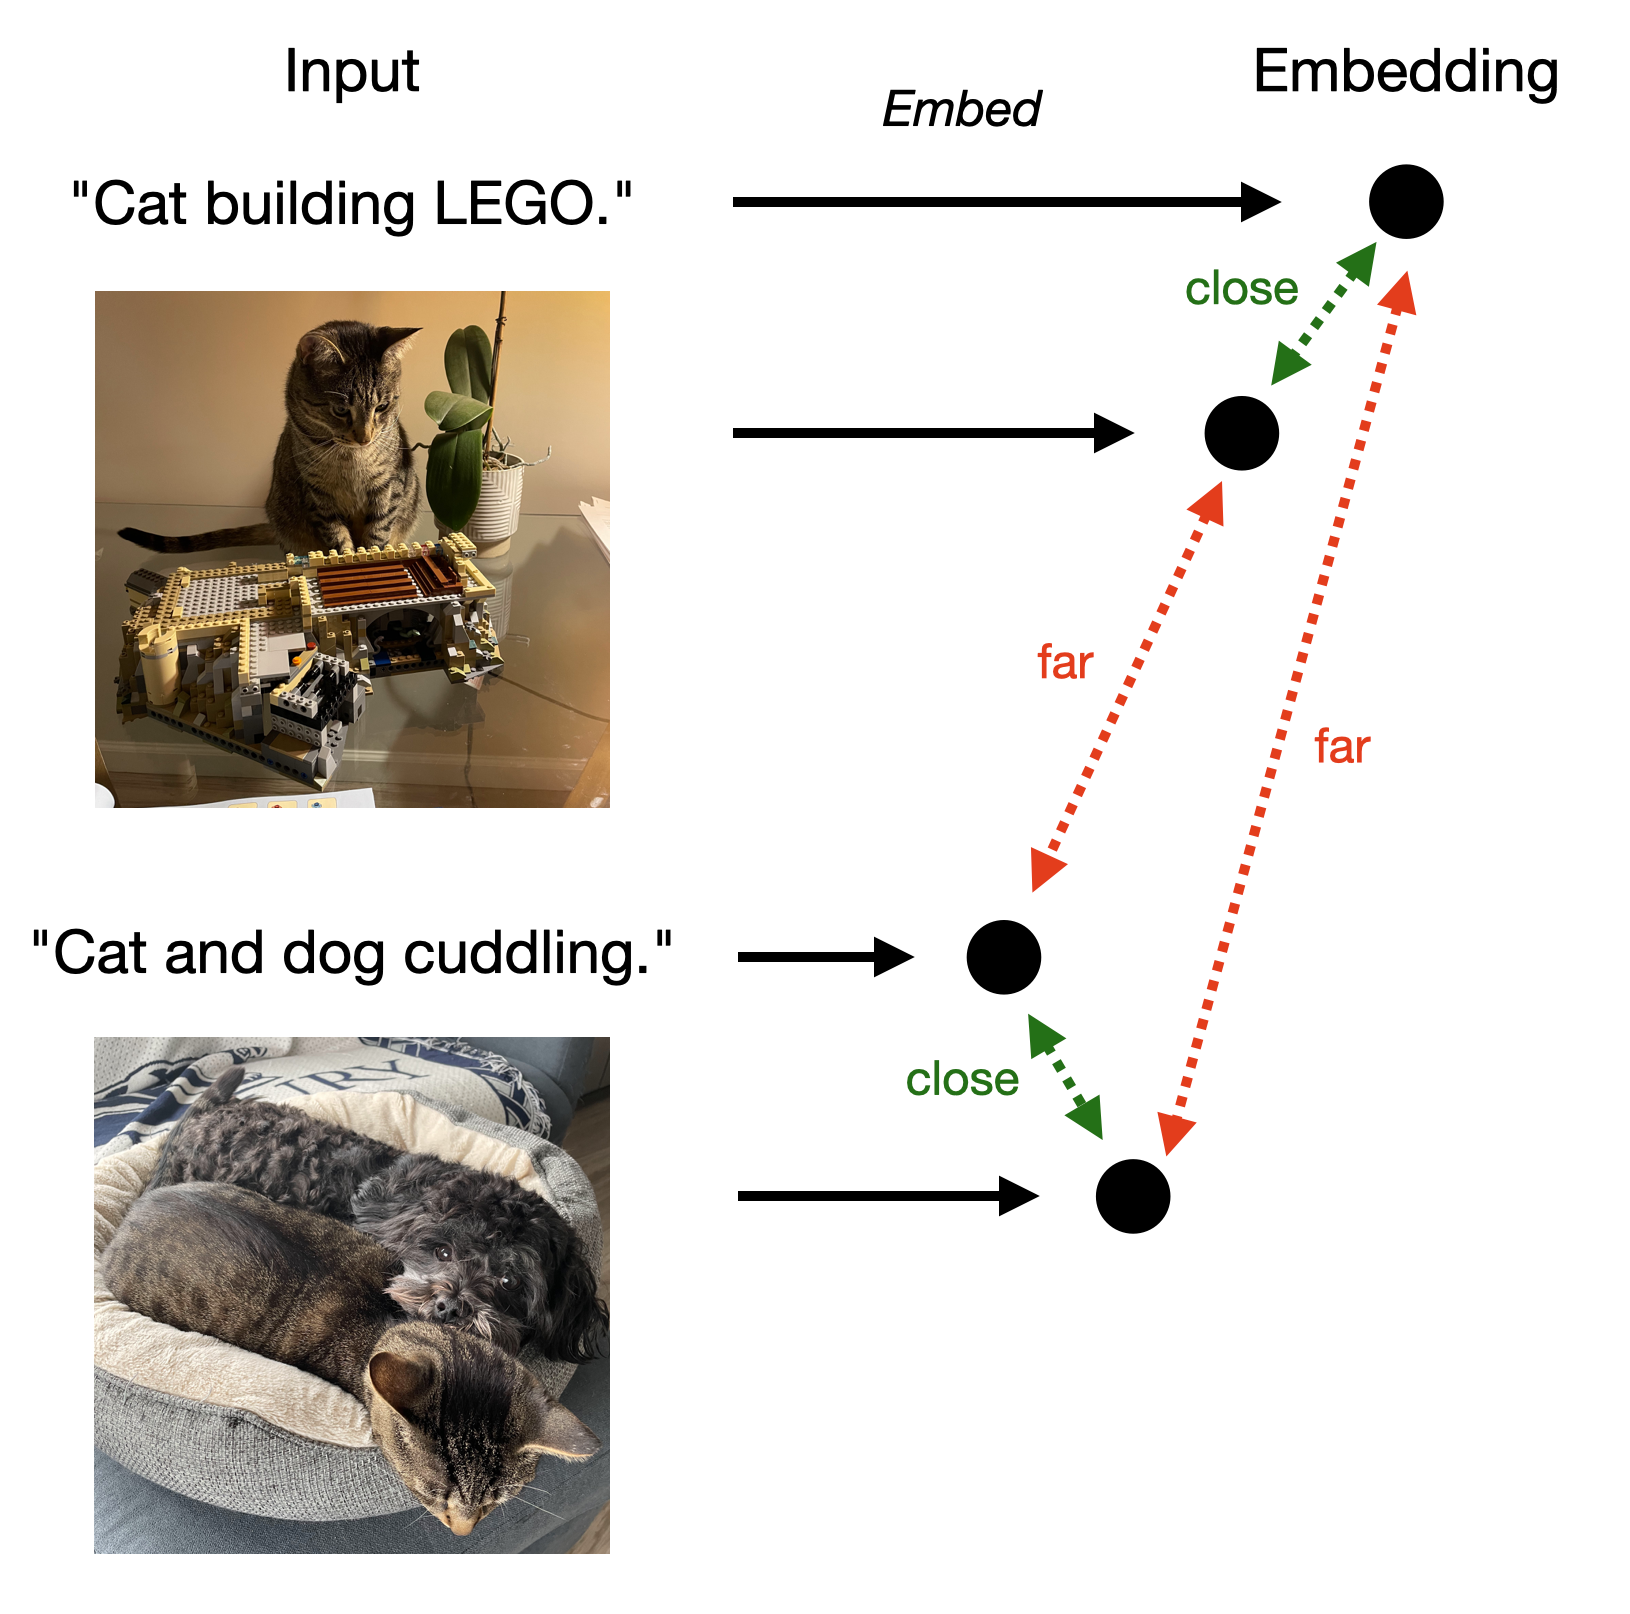
\includegraphics[width=0.55\textwidth]{IMAGES/contrastive_CLIP.png}
    \caption[Illustration of Contrastive Learning]{Illustration of Contrastive Learning. Source:v7labs\footnotemark.}
    \label{fig:contrastive_learning}
\end{figure}
\footnotetext{\url{https://www.v7labs.com/blog/contrastive-learning-guide}}
\subsubsection{Contrastive Loss Function}
The contrastive loss function is formulated as follows:

\begin{equation}
\mathcal{L} = -\log \frac{\exp(\text{sim}(q, k^+))}{\sum_{k \in K} \exp(\text{sim}(q, k))}
\end{equation}
where:
\begin{itemize}
    \item \( q \) is the embedding of an anchor (e.g., an image encoded by a function \( f \)).
    \item \( k^+ \) is the embedding of a positive example (e.g., a corresponding text encoded by function \( g \)).
    \item \( K \) includes both the positive example and a set of negative examples \( k^- \).
    \item \( \text{sim}(q, k) \) denotes a similarity measure, such as cosine similarity.
    \item The negative log ensures that the similarity between \( q \) and \( k^+ \) is maximized while pushing away the negative examples \( k^- \).
\end{itemize}


% CHAPTER 3
\pagestyle{fancy}
\chapter{Quantization Techniques}
\label{chap:Vector quantization in VBDMS}
This chapter explores \textbf{vector quantization} techniques, which arise from the need to optimize the memory and disk footprint of \textbf{VDBMS}. By reducing storage requirements, these techniques enable more efficient resource usage and higher \textbf{queries per second (QPS)}. However, this efficiency comes at the expense of search accuracy, introducing a trade-off between precision and performance. Quantization methods can be broadly categorized into two types: those that reduce dimensionality, such as \textbf{Product Quantization}, and those that approximate values, such as \textbf{Scalar Quantization} and \textbf{Binary Quantization}.

\section{Product Quantization}
\textbf{Product Quantization (PQ)} reduces memory usage by restricting vector representation, making storage and retrieval more efficient. The process begins by dividing the original vector into several smaller sub-vectors of equal size, and the greater the number of sub-vectors, the lower the compression rate, as more data points need to be stored. Each sub-vector represents a separate subspace, where we apply a clustering algorithm associated with its closest centroid.
\begin{figure}[h]
    \centering
    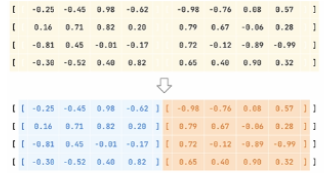
\includegraphics[width=0.5\textwidth]{IMAGES/immagine_2025-02-27_122846884.png}
    \caption{Product Quantization. Source: DeepLearning.AI.\footnotemark[1]}
    \label{fig:PQ}
\end{figure}
\footnotetext[1]{\url{https://learn.deeplearning.ai/courses/retrieval-optimization-from-tokenization-to-vector-quantization/lesson/1/introduction}}

\begin{description}
\item[\textbf{Codebook}:] It refers to the collection of all centroids of a specific subspace.
\end{description}

Formally, the \textbf{product quantization} process goes as follows:
\begin{enumerate}
    \item Decomposing the vector \( \mathbf{x} \) into subvectors \( k \): \( \mathbf{x} = [\mathbf{x}_1, \mathbf{x}_2, \dots, \mathbf{x}_k] \), where each subvector \( \mathbf{x}_i \in \mathbb{R}^{d_i} \) and \( \sum_{i=1}^k d_i = d \).
    \item Quantizing each sub-vector \( \mathbf{x}_i \) independently using a \textbf{codebook} \( C_i = \{c_{i1}, c_{i2}, \dots, c_{iM}\} \), where \( M \) is the number of centroids for each sub-vector.
    \item The quantized vector is then the concatenation of the indices of the chosen codewords: \( \mathbf{q} = [q_1, q_2, \dots, q_k] \), where \( q_i \) is the index of the nearest codeword in \( C_i \).
\end{enumerate}


\subsection{Centroid Generation}
As for generating centroids, VDBMSs like Weaviate and Qdrant rely on the widely used encoder algorithm \textbf{K-means}. It defines a \textbf{K} parameter, which is the number of partitions (also referred to as tiles) we want for our subvector space. The algorithm starts by assigning \textbf{K} random centroids within the dataset, then iteratively assigns the closest vectors to them, recalculating the cluster using the mean of the residing vectors. The algorithm stops when the centroids have stabilized or a maximum number of iterations have been reached.
\begin{figure}[h]
    \centering
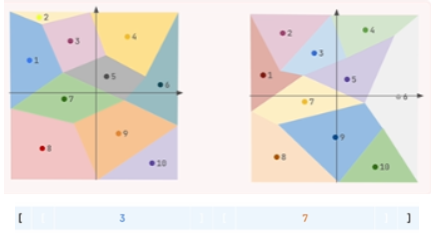
\includegraphics[width=0.6\textwidth]{IMAGES/immagine_2025-02-27_123033735.png}
    \caption{Partitioned Vector Space. Source: DeepLearning.AI.\footnotemark[1]}
    \label{fig:PQ}
\end{figure}
Another algorithm used to partition the subvector space is the \textbf{Tile encoder}. This algorithm aims to resolve one of the main limitations of K-means, which is the tendency for centroids to become outdated over time as new vectors join the collection. This results in some centroids becoming more populated than others. 

The Tile encoder addresses this issue by employing the Cumulative Density Function (CDF), denoted as \textbf{CDF}(x). Given our data collection, it returns the probability (a value from 0 to 1) that a data point is less than or equal to \(x\). Using the formula \(\text{code}(x) = \text{CDF}(x) \times c\) (where c is the number of codes/clusters we need), we determine the cluster to which the data point \(x\) belongs. 


\section{Scalar Quantization}
\textbf{Scalar Quantization} reduces the precision of numerical values by mapping continuous floating-point numbers to a fixed set of discrete levels. Typically, this involves converting each dimension from a 32-bit floating-point representation to an 8-bit integer. The process begins by analyzing the data to determine the range, setting boundaries based on the minimum and maximum values from a training set. The range is then divided into a fixed number of intervals (e.g., 256 for 8-bit quantization), with each value assigned to the nearest bucket. The resulting integer represents the corresponding bucket, enabling a more compact and efficient representation while preserving as much information as possible within the given bit constraint.
\begin{figure}[h]
    \centering
    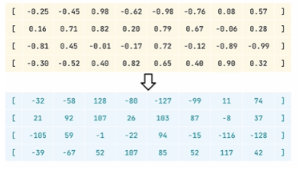
\includegraphics[width=0.5\textwidth]{IMAGES/immagine_2025-02-27_123316646.png}
    \caption{Scalar Quantization. Source: DeepLearning.AI.\footnotemark[1]}
    \label{fig:SQ}
\end{figure}

\section{Binary Quantization}
\textbf{Binary Quantization} consists of converting a floating point to a binary representation, taking the quantization to the extreme by transitioning from a 32-bit representation to a single bit. By sacrificing a huge amount of information and distance calculation accuracy, \textbf{Binary Quantization} excels by having a minor memory and disk footprint. This technique is very susceptible to \textbf{oversampling}(vectors with the same compressed representation), while being the fastest.
\begin{figure}[h]
    \centering
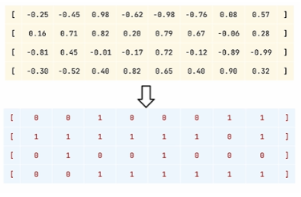
\includegraphics[width=0.5\textwidth]{IMAGES/immagine_2025-02-27_123438887.png}
    \caption{Binary Quantization. Source: DeepLearning.AI.\footnotemark[1]}
    \label{fig:BQ}
\end{figure}

\section{Overfetching and Rescoring}
To mitigate the limitations of vector quantization, vector database management systems (\textbf{VDBMSs}) employ \textbf{overfetching} and \textbf{rescoring}. Due to the lossy nature of quantization, multiple vectors may share the same compressed representation, leading to potential collisions.
To address this, databases like Weaviate use \textbf{overfetching}, retrieving a larger set of candidates instead of selecting only the top-$K$ results from the quantized index. This ensures that relevant matches are not overlooked. Once these compressed vectors are retrieved, \textbf{rescoring} is performed by fetching the original, high-precision vectors from disk. The query is then re-evaluated against this smaller subset, improving accuracy while maintaining search efficiency.
\begin{figure}[h]
    \centering
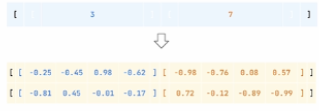
\includegraphics[width=0.5\textwidth]{IMAGES/immagine_2025-02-27_123548078.png}
    \caption{Example of vectors with the same quantized representation. Source: DeepLearning.AI.\footnotemark.}
    \label{fig:Overfetching}
\end{figure}
\footnotetext{\url{https://learn.deeplearning.ai/courses/retrieval-optimization-from-tokenization-to-vector-quantization/lesson/1/introduction}}
\section{Memory Impact of Quantization in Vector Databases}
Quantization optimizes memory usage in large-scale vector databases by reducing precision. Common techniques include:
\begin{itemize}
    \item \textbf{Scalar Quantization (SQ):} Converts 32-bit floating-point values to 8-bit integers, reducing storage size by a factor of 4.
    \item \textbf{Product Quantization (PQ):} Splits vectors into subvectors, assigns each to a centroid, and stores them as small fixed-size codes (e.g., 1-byte indices). This significantly reduces memory usage but increases indexing complexity.
    \item \textbf{Binary Quantization:} Maps floating-point values to a single bit per value, maximizing compression but sacrificing accuracy.
\end{itemize}

By default, an \textbf{OpenAI embedding} with 1,536 dimensions requires approximately \textbf{6KB per vector}. Applying \textbf{SQ} reduces this to \textbf{1.5KB}, while \textbf{PQ} achieves \textbf{10x or greater compression}, balancing memory efficiency with computational overhead and potential precision loss. The choice of quantization technique depends on the trade-off between storage savings, search latency, and retrieval accuracy.
\section{Experimentation with the quantization techniques}
The Figures below show the disk storage impact and query performance across different embedding formats for the Paper dataset, which consists of 2 million vectors (200 dimensions, float32) evaluated over 100k queries. The experiment has been performed on the VDBMS Weaviate.
\begin{figure}[h]
    \centering
    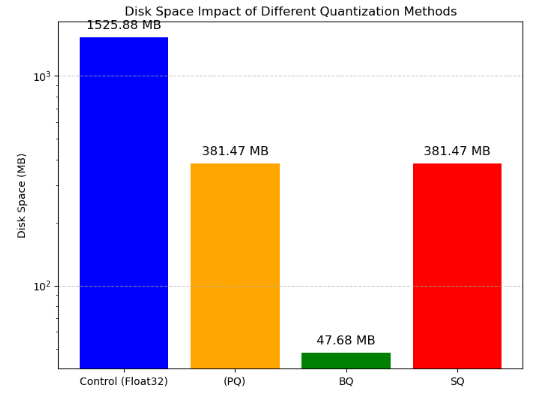
\includegraphics[width=0.4\textwidth]{IMAGES/immagine_2025-02-25_105819873.png}
    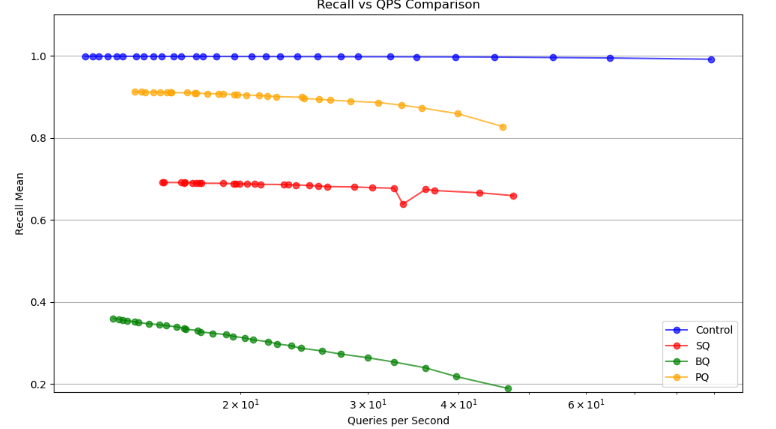
\includegraphics[width=0.4\textwidth]{IMAGES/immagine_2025-02-25_105043241.png}
    \caption{Disk usage and performance difference between the different techniques.}
    \label{fig:Disk Impact}
\end{figure}










\chapter{Indexes}
\label{chap:Indexes in VBDMS}
This chapter will shed light on the indexing aspect of Vector Database Management Systems, specialized data structures that intelligently organize vectors by leveraging their mathematical properties. Their purpose is to optimize the retrieval process that assists search algorithms by improving their performance. There is no index that is tailored for all use cases; each index has been designed with their advantage and disadvantages, the only thing that different approaches have in common is to assist (especially in the large-scale context) reducing the search complexity to sublinear levels.

\section{Flat Index}
The flat index is the simplest approach for vector storage; it involves storing the vectors directly, meaning that queries are always an exact k-nearest neighbors (kNN) search, where the query vector is compared to every other vector in the collection. This approach has limited scalability, as the search speed begins to decline as the vector collection grows. The flat index is best suited for use cases with a manageable collection size, where search accuracy takes priority over search speed.

\section{LSH with Random Projection}
The Locality-Sensitive Hashing (LSH) indexing technique maps high-dimensional vectors to low-dimensional representations by leveraging hash functions that preserve locality and distribution. Vectors that are close in the original space are more likely to share the same hash value. This approach intentionally creates collisions to facilitate efficient retrieval of similar vectors, using hyperplanes as partitioning boundaries.
\begin{figure}[h]
    \centering
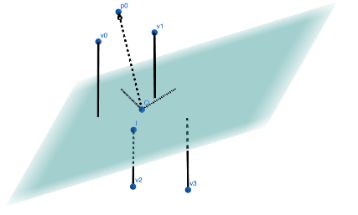
\includegraphics[width=0.35\textwidth]{IMAGES/immagine_2025-02-27_130242965.png}
    \caption{Example of Hyperplane. Source: Sofrwaredoug.\footnotemark.}
    \label{fig:Random Projection}
\end{figure}
\footnotetext{\url{https://softwaredoug.com/blog/2023/08/21/implementing-random-projections}}
\end{figure}
A hyperplane splits the vector space into two regions: a positive side and a negative side. To determine which side a vector resides on, the dot product between the vector and a normal vector (perpendicular to the hyperplane) is computed.

The dot product of two vectors $\vec{a} = (a_1, a_2, \dots, a_n)$ and $\vec{b} = (b_1, b_2, \dots, b_n)$ is:

\[
\vec{a} \cdot \vec{b} = \sum_{i=1}^{n} a_i b_i = a_1b_1 + a_2b_2 + \dots + a_nb_n
\]

\begin{itemize}
    \item If the dot product is \textbf{positive}, the vector is assigned a label of \textbf{1} (positive side).  
    \item If the dot product is \textbf{negative}, the vector is assigned a label of \textbf{0} (negative side).  
\end{itemize}

By applying multiple hyperplanes, we create a hashed representation of vectors as binary sequences (composed of 0s and 1s), significantly reducing storage requirements. With $N$ random hyperplanes, each vector is represented as an $N$-bit binary code indicating on which side of each hyperplane it falls.

To measure similarity between vectors, we compute their \textbf{Hamming distance}, which is the number of differing bits between their binary codes.  
\begin{itemize}
    \item A Hamming distance of \textbf{0} indicates that both vectors fall into the same region, meaning no hyperplane separated them.  
    \item Larger Hamming distances indicate greater dissimilarity.
\end{itemize}

Additionally, random projections can be visualized as an \textbf{LSH Tree}, where each hyperplane acts as a decision node, branching into two possible paths: positive or negative. Traversing the tree based on these binary splits results in an efficient search structure for approximate nearest-neighbor queries.

\section{Inverted File Index (IVF)}
The \textbf{Inverted File Index} (IVF) is an indexing technique designed to enhance Approximate Nearest Neighbor (ANN) search performance. IVF partitions the vector space into centroids and limits searches to specific regions, making it ideal for large-scale, high-dimensional applications.

\subsection{Clustering and Voronoi Cells}
A predefined number of centroids is established before clustering, creating an inverted index that associates each vector with its nearest centroid. Once clustering is complete, clusters expand until they form \textit{Voronoi cells}, where each vector belongs to a single cell, defined by the shortest distance to its centroid.
\begin{figure}[h]
    \centering
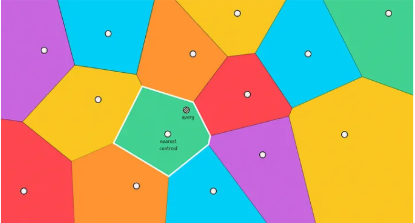
\includegraphics[width=0.55\textwidth]{IMAGES/immagine_2025-02-27_130909576.png}
    \caption{Example of Voronoi cells. Source: Towardsdatascience.\footnotemark[2]}
    \label{fig:Voronoi}
\end{figure}
\footnotetext[2]{\url{https://towardsdatascience.com/similarity-search-knn-inverted-file-index-7cab80cc0e79}}
\subsection{Querying and the Edge Problem}
Queries locate the nearest centroids and search for the closest vectors within them. However, the \textbf{edge problem} arises when suitable vectors near Voronoi boundaries are ignored. This issue worsens in high dimensions as cell boundaries become less distinct. To mitigate this, querying multiple cells increases recall at the cost of speed.
\begin{figure}[h]
    \centering
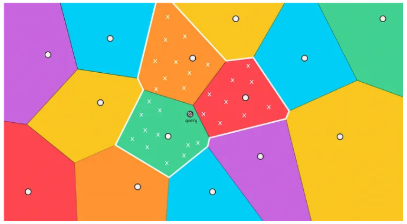
\includegraphics[width=0.55\textwidth]{IMAGES/immagine_2025-02-27_131611893.png}
    \caption{Edge problem. Source: Towardsdatascience.\footnotemark[2]}
    \label{fig:VoronoiEdges}
\end{figure}
\subsection{IVF Variants}
The basic form of IVF, known as \textbf{IVFFlat}, performs a brute-force search within identified cells. Advanced variants such as \textbf{IVFPQ} (Product Quantization) and \textbf{IVFSQ} (Scalar Quantization) compress vector representations, enhancing scalability and reducing memory usage. These techniques will be covered in the next chapter.


\section{Navigable Small Worlds}
The NSW index consists of a graph that contains both long-range and short-range links. It is based on the “small world” or "six degrees of separation" rule, where each entity is, on average, separated by six degrees of link separation. This structure exhibits a high degree of clustering, where nodes are grouped into tightly-knit communities, yet only a few steps are needed to traverse between two different nodes. Essentially, this allows nodes that are typically "far" from each other in other graph-based structures to reach one another in just a few steps. Each node represents an item and maintains a friend list containing other vertices to which it is connected. This solution is fast but not highly accurate and requires tuning to perform well in ANN search over high-dimensional spaces.

\subsection{Construction}
Unlike some other indexes, the construction of the index is not a deterministic process, at first the dataset is shuffled and then the nodes are sequentially created. The main parameters in this process is  \textbf{M} which the maximum number of connections a node can have. As nodes are inserted it gets connected to nearest nodes based on a distance metrics like the cosine distance.

\begin{figure}[h]
    \centering
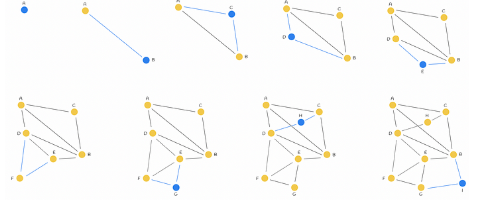
\includegraphics[width=0.55\textwidth]{IMAGES/immagine_2025-02-27_132644429.png}
    \caption{Example of NSW construction with M=2. Source: Towardsdatascience.\footnotemark.}
    \label{fig:NSW}
\end{figure}
\footnotetext{\url{https://www.deeplearning.ai/short-courses/vector-databases-embeddings-applications/ }}

\subsection{Graph traversal}
The search begins by selecting a vertex as the entry point. It then performs a greedy search, determining the next vertex to move to by checking the current vertex’s friend list and moving to the closest vertex to the query node. The search terminates when no closer node is found.  
Since this search strategy is inherently greedy, it attempts to reach the global optimal solution by making the best local decision at each step. While this approach is simple and fast, it is susceptible to early stopping, where the search gets trapped in regions of the graph where the local optimum has no better neighboring candidates.  
To mitigate the risk of getting stuck in dead regions, various strategies can be employed. One such method is \textbf{“beam search"}, which maintains a \textbf{top-k} list of the best candidates at each step. Another approach is “multi-hop search,” which considers not only direct neighbors but also neighbors of neighbors.
\begin{figure}[h]
    \centering
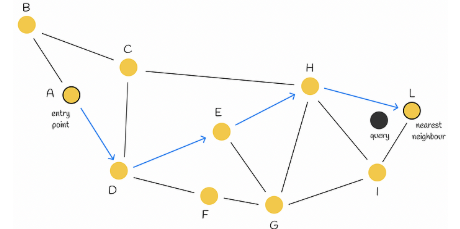
\includegraphics[width=0.6\textwidth]{IMAGES/immagine_2025-02-27_132919654.png}
    \caption{example of NSW routing where A is entry point. Source: DeepLearningAI.\footnotemark.}
    \label{fig:NSW traversal}
\end{figure}
\footnotetext{\url{https://www.deeplearning.ai/short-courses/vector-databases-embeddings-applications/ }}

\section{Hierarchical Navigable Small Worlds}
The HNSW index is an evolution of the \textbf{Navigable Small World (NSW)} graph, incorporating principles from the probabilistic data structure known as the \textbf{skip list}. A skip list consists of multiple layers of ordered linked lists, where each upper layer contains a subset of elements from the layer below. This hierarchical structure enables efficient search by starting from the topmost layer and performing a sequential search.  
\begin{figure}[h]
    \centering
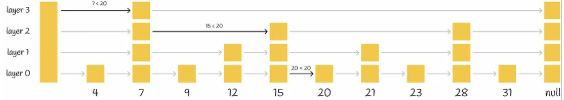
\includegraphics[width=0.8\textwidth]{IMAGES/immagine_2025-02-27_133448847.png}
    \caption{Skip List. Source: Towardsdatascience.\footnotemark[2]}
    \label{fig:Skip List}
\end{figure}

If the target element is found, the search terminates. Otherwise, upon encountering a greater value, the algorithm descends to the next layer, using the previously visited element as the new entry point.  


The \textbf{HNSW} index follows a similar layered structure, where:
\begin{itemize}
    \item The \textbf{topmost layer} contains a small subset of representative nodes.
    \item The \textbf{in-between layers} contain progressively more nodes.
    \item The \textbf{lowest layer} includes all nodes in the dataset.
\end{itemize}
\begin{figure}[h]
    \centering
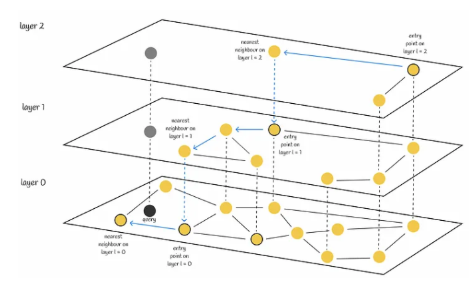
\includegraphics[width=0.7\textwidth]{IMAGES/immagine_2025-02-27_133909960.png}
    \caption{HNSW index. Source: Towardsdatascience.\footnotemark[2]}
    \label{fig:HNSW}
\end{figure}
This multi-layered organization significantly improves retrieval efficiency by reducing the number of comparisons required for nearest neighbor search.  

\subsection{Search Process}  

The HNSW query process is similar to NSW but introduces a hierarchical search mechanism. After locating the nearest node in a layer, it serves as the entry point for the lower layer.  

HNSW graphs follow the skip list principle:  
\begin{itemize}  
    \item The \textbf{topmost layer} has fewer nodes and connections.  
    \item Lower layers have increasing connectivity until \textbf{Layer 0}, which contains all data points.  
\end{itemize}  

The search begins at a predefined entry node in the top layer and performs a greedy search. The algorithm descends to the next layer when it finds a closer node in that layer. This process continues until reaching Layer 0, ensuring all potential nearest neighbors are considered.  

HNSW search is controlled by key parameters:  
\begin{itemize}  
    \item \textbf{$ef$ (exploration factor)}: Determines the number of candidate nodes kept during the search. A higher $ef$ improves recall at the cost of increased latency. 
    \item \textbf{Entry Point Selection}: The algorithm selects a fixed or dynamically chosen entry node in the topmost layer to begin the search.  
\end{itemize}  

These parameters allow fine-tuning of search accuracy, efficiency, and resource usage in HNSW-based vector searches.  
\subsubsection{Impact of M parameter on HNSW search}
The Figures below show the impact of different values of M,performed over the embedding that come from the Tripclick dataset, which consists rhoughly of 800k vectors (768 dimensions, float32) evaluated over 1000 queries. The experiment has been performed on the VDBMS Weaviate.
\begin{figure}[h]
    \centering
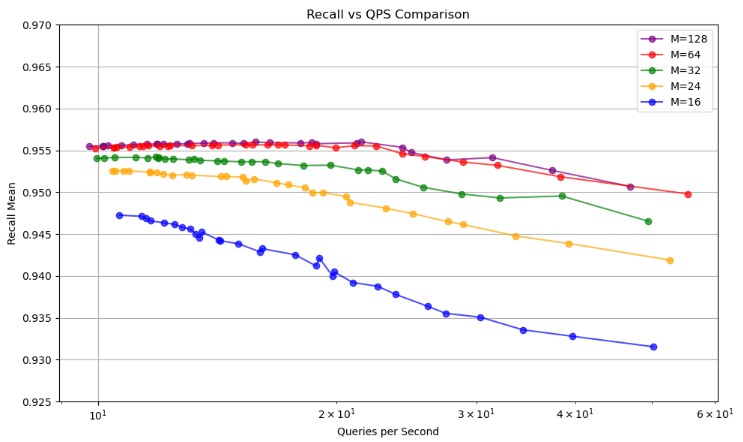
\includegraphics[width=0.7\textwidth]{IMAGES/immagine_2025-02-27_142057404.png}
    \caption{QPS vs Recall between different values of M.}
    \label{fig:M search}
\end{figure}

\subsection{Construction Process of HNSW}
The construction of an \textbf{HNSW} index follows a hierarchical approach, inspired by skip lists, to optimize approximate nearest neighbor search. The graph is built incrementally, adding one data point at a time while maintaining efficient connectivity across multiple layers.
\subsubsection*{Key Parameters}
The construction process is governed by several key parameters:
\begin{itemize}
    \item \textbf{Maximum Layer ($L_{\max}$):}  
    Determines the highest level a node can be assigned. It is typically chosen using a logarithmic distribution based on the dataset size.

    \item \textbf{Maximum Connections per Layer ($M$):}  
    Defines the number of bidirectional edges each node can maintain per layer, balancing search efficiency and memory usage.

    \item \textbf{Connectivity Factor (efConstruction):}  
    Controls the number of nearest neighbors considered during graph construction. A higher value results in better graph quality but increases indexing time.

    \item \textbf{Insertion Strategy:}  
    Each new data point is assigned a random layer up to $L_{\max}$ and inserted into the graph by connecting to its $M$ nearest neighbors in each layer.

    \item \textbf{Pruning Strategy:}  
    Redundant edges are removed to ensure efficient navigation while maintaining strong graph connectivity.
\end{itemize}

\subsubsection*{Construction Algorithm}

\begin{enumerate}
    \item Assign each new data point a layer up to $L_{\max}$.
    \item Insert the point into the topmost layer and connect it to the $M$ nearest neighbors.
    \item Repeat the process for each lower layer, ensuring bidirectional edges.
    \item Apply pruning to maintain an optimal balance between connectivity and efficiency.
\end{enumerate}

The hierarchical structure ensures that higher layers facilitate fast exploration, while lower layers refine the search for precise nearest neighbors.


 
\section{DiskANN}
One of the main drawback of graph-based indexes like NSW and HNSW, is the significant memory footprint, which makes querying over large amount of data expensive. While this may not be an issue in distributed and high resources environments, the same cannot be said for single machines with limited memory. The most basic approaches for handling single node environments are the employment of \textbf{IVFPQ} or by sharding the dataset with their own in-memory indexes which during the search each result is merged together. These solution suffer from a lower recall and to address this, \textbf{DiskANN} provides an SSD resident index with the objective of reducing the memory footprint and optimize disk accesses thanks to the assistance of the \textbf{Vamana} algorithm, which differentiates itself from NSW by constructing the graph in order to optimize disk access instead of improved traversal.

\subsection{Graph Construction Process}
Instead of starting with a sparse graph and gradually adding edges (as in NSW), Vamana begins with a dense graph and iteratively prunes unnecessary edges. The process consists of the following steps:

\begin{enumerate}
    \item \textbf{Initialize:}  
    Start with a randomly connected graph with excess edges.  

    \item \textbf{Graph Construction:}  
    For each point $p$:  
    \begin{enumerate}
        \item \textbf{Find Nearest Neighbors:} Greedy search in the current graph.  
        \item \textbf{Prune Edges:} Remove redundant connections while ensuring connectivity.  
        \item \textbf{Add Backward Links:} Ensure bidirectional edges for efficient traversal.  
    \end{enumerate}

    \item \textbf{Refinement:}  
    Perform two rounds of pruning with different distance thresholds to optimize local and long-range connections.  

    \item \textbf{Disk Optimization:}  
    Store the graph efficiently to minimize random disk access and enable batched reads.  
\end{enumerate}
This pruning-based method enables Vamana to optimize the trade-off between \textbf{graph diameter}, which influences search depth, and \textbf{node degree}, which impacts memory consumption, more efficiently than conventional techniques. DiskANN utilizes Vamana because it builds a \textbf{flat graph}, making it more suitable for disk storage compared to hierarchical structures.
\begin{figure}[h]
    \centering
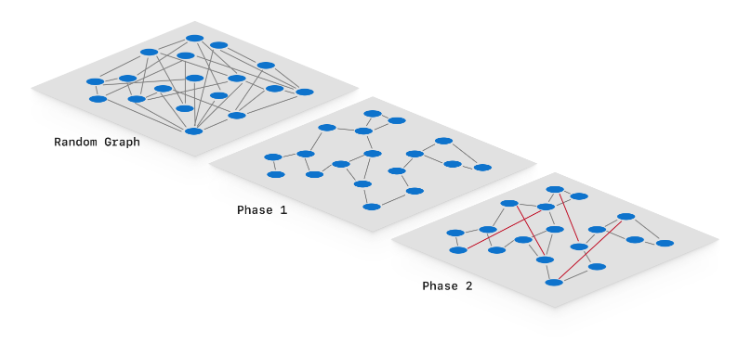
\includegraphics[width=0.7\textwidth]{IMAGES/immagine_2025-02-27_134619701.png}
    \caption{Vamana Graph example. Source: Planetscale.\footnotemark.}
    \label{fig:Vamana}
\end{figure}
\footnotetext{\url{https://planetscale.com/docs/vectors/terminology-and-concepts
}}
\subsection{Optimizations in DiskANN}
DiskANN provides some optimization in order to increase querying performance:

\begin{itemize}
    \item \textbf{Caching:} Nodes that are fetched more freqeuntly than others are stored in RAM, in order to reduce SSD use and increase the performance.
    \item \textbf{Compressed vectors and re-ranking:} In order to increase retrieval efficiency, vectors are stored in RAM in their compressed form, in order to do a preliminary comparison. After, a re-ranking process is done with a full precision SSD search.
    \item \textbf{Clustered Indexing:} Partitions data into overlapping clusters using k-means clustering. Each data point belongs to multiple clusters, ensuring connectivity for search algorithms.
    \item \textbf{Beam Search:} Retrieves neighborhood data from SSD in small batches, reducing read latencies by grouping nearby data access requests.
\end{itemize}

% CHAPTER 5
\pagestyle{fancy}
\chapter{Query processing}
\label{chap:Query processing}
\pagestyle{fancy}

Query processing in a vector database is the process of searching for the most relevant results from a collection of vectors. It starts with a search specification, which includes a similarity score and the type of query; all of these are provided by users through a query interface.
After receiving the query, the system processes it by running a series of steps in the vector collection. These steps include simple similarity searches and faster methods that use indexes to improve efficiency. This ensures that the search is handled quickly and returns accurate results.
\section{Vector similarity search}
The goal of a vector similarity search is to efficiently identify vectors that are most similar to a given query vector based on a specified distance or similarity metric. This search process is often used in high-dimensional spaces, where traditional search techniques can become computationally expensive. Several types of vector similarity search techniques exist, each with its trade-offs in terms of accuracy, efficiency, and applicability to different problems.
\subsection{Distance metrics}
Vector similarity search leverages the mathematical properties of vectors to find the most relevant vectors in a database in response to a query. This is done by evaluating the distance metric between the query vector \textbf{q} and the vectors \textbf{v} in the database. A distance score, often denoted \textbf{d(q,v)}, calculates a scalar value of the two \textbf{D}-dimensional vectors, where a smaller value indicates greater similarity between the vectors. The vectors with the lowest distance scores are considered the most similar to the query vector.

\begin{itemize}
    \item \textbf{Euclidean Distance:} Measures the straight-line distance between two points in a D-dimensional space.
    \[
    d(a, b) = \sqrt{\sum_{i=1}^{D} (a_i - b_i)^2}
    \]
    \item \textbf{Manhattan Distance (L1 Norm):} Calculates the sum of absolute differences between the coordinates of two vectors.
    \[
    d(a, b) = \sum_{i=1}^{D} |a_i - b_i|
    \]
    \item \textbf{Cosine Similarity:} Computes the cosine of the angle between two vectors, often used as a similarity metric. The corresponding distance is:
    \[
    d(a, b) = 1 - \frac{\sum_{i=1}^{D} a_i b_i}{\sqrt{\sum_{i=1}^{D} a_i^2} \sqrt{\sum_{i=1}^{D} b_i^2}}
    \]
    \item \textbf{Jaccard Distance:} Used for binary or sparse data, defined as:
    \[
    d(a, b) = 1 - \frac{|a \cap b|}{|a \cup b|}
    \]
    \item \textbf{Hamming Distance:} Calculates the number of positions where two binary vectors differ.
    \[
    d(a, b) = \sum_{i=1}^{D} \mathbb{I}(a_i \neq b_i)
    \]
\end{itemize}
\subsection{KNN}
The K Nearest Neighbor algorithm is the most straightforward approach when it comes to Vector Similarity Search, providing an exact result by confronting the k nearest vectors in the vector space. Although this brute-force algorithm provides perfect recall, it requires a lot of computation resources, and, by consequence, the query runtime increases along as the number of data points increases. 
\subsection{ANN}
The Approximate Nearest Neighbor (ANN) algorithm was developed to address the limitations of the k nearest neighbors (kNN) approach, particularly its inefficiency when scaling to large datasets. The primary goal of ANN is to provide near-optimal results while significantly reducing computation time compared to exact kNN searches. Using techniques that approximate nearest neighbors, ANN enables the handling of massive collections of vectors, offering a practical solution for high-dimensional search tasks. The ANN approach also makes use of the vector indexes such as NSW and HNSW that are based on the concept of "six degrees of separation" allowing the algorithm to explore the vector space more efficiently.

\section{Performance metrics}
Assessing the quality of the vector similarity search requires the definition of clear and relevant performance metrics. These metrics provide a standardized way to measure how effectively the search algorithm retrieves the most relevant results from the vector collection, and allows one to find which approach is more suitable for a specific use case.
\begin{itemize}
    \item \textbf{Precision:} Measures the proportion of relevant results among the retrieved results.
    \[
    \text{Precision} = \frac{\text{Number of Relevant Results Retrieved}}{\text{Total Number of Results Retrieved}}
    \]

    \item \textbf{Recall:} Measures the proportion of relevant results that were successfully retrieved.
    \[
    \text{Recall} = \frac{\text{Number of Relevant Results Retrieved}}{\text{Total Number of Relevant Results in the Database}}
    \]
    \item \textbf{Queries Per Second (QPS):} Measures the system's throughput by calculating the number of queries processed per second.
    \[
    \text{QPS} = \frac{\text{Number of Queries Processed}}{\text{Total Time (in seconds)}}
    \]
\end{itemize}


\section{Filtering Techniques}
Filtering techniques in vector search help refine results based on predefined criteria. These techniques ensure that retrieved documents meet specific conditions, improving relevance and accuracy.

\subsection{Pre-filtering}
Pre-filtering applies constraints before executing the search query. This method reduces the search space, leading to faster retrieval times. Common pre-filtering techniques include:
\begin{itemize}
    \item Applying metadata filters (e.g., date, category, author).
    \item Restricting searches to specific document subsets.
    \item Leveraging user-defined conditions for search optimization.
\end{itemize}
\begin{figure}[h]
    \centering

\includegraphics[width=0.8\textwidth]{IMAGES/immagine_2025-03-03_093943770.png}
    \caption[Pre-filtering]{Pre-filtering process. Source: Weaviate\footnotemark[1]}
    \label{fig:Rectangle Tree}
\end{figure}
\footnotetext[1]{\url{https://weaviate.io/blog/speed-up-filtered-vector-search}}
\subsection{Post-filtering}
Post-filtering applies constraints after the search query has been executed. This approach ensures that filtering does not interfere with similarity computations. Common post-filtering techniques include:
\begin{itemize}
    \item Removing results that do not meet certain thresholds.
    \item Applying additional business logic to refine search outputs.
    \item Filtering based on dynamic user preferences after initial retrieval.
\end{itemize}
\begin{figure}[h]
    \centering

\includegraphics[width=0.8\textwidth]{IMAGES/immagine_2025-03-03_094158324.png}
    \caption[Post-filtering]{Post-filtering process. Source: Weaviate\footnotemark[1]}
    \label{fig:Rectangle Tree}
\end{figure}
\subsection{In-filtering}
In-filtering integrates filtering conditions directly into the similarity computation process. This technique ensures that relevance scoring inherently considers filtering constraints. Key aspects of in-filtering include:
\begin{itemize}
    \item Modifying similarity calculations to account for filtering parameters.
    \item Embedding constraints within vector representations.
    \item Ensuring efficient and scalable implementation in high-dimensional spaces.
\end{itemize}

\section{ACORN}
ACORN is a predicate-agnostic hybrid search method that extends HNSW to efficiently handle structured query filters. Unlike traditional pre-filtering and post-filtering methods, ACORN achieves sublinear retrieval times even with high-cardinality predicate sets. It constructs a denser graph index and applies predicate-aware traversal strategies to optimize search performance. By leveraging efficient predicate-subgraph traversal while maintaining the speed advantages of HNSW, ACORN provides a scalable and high-performance alternative to traditional hybrid search strategies.

Key parameters governing ACORN's behavior include:
\begin{itemize}
    \item $\gamma$: Neighbor expansion factor.
    \item $M_{\beta}$: Compression parameter for neighbor pruning.
    \item $M$: Degree bound for traversed nodes.
    \item $e$: Fixed entry point to the index.
    \item $s_{min}$: Minimum predicate selectivity.
\end{itemize}

\subsection{Index Construction}
The ACORN-$\gamma$ index is built using two key modifications to HNSW:
\begin{enumerate}
    \item \textbf{Neighbor List Expansion:} Each node collects $M \cdot \gamma$ approximate nearest neighbors instead of the standard $M$. This ensures that filtering operations during search do not fragment the graph.
    \item \textbf{Predicate-Agnostic Pruning:} To counter increased index size, a compression heuristic is applied to bottom-level neighbor lists, reducing memory overhead while maintaining navigability.
\end{enumerate}
A recommended choice for $\gamma$ is $1/s_{min}$, ensuring efficient pre-filtering when selectivity drops below $s_{min}$. This enables ACORN to balance indexing cost and search efficiency.

\subsection{Search Algorithm}
ACORN employs a hierarchical greedy search similar to HNSW but integrates predicate filtering:
\begin{enumerate}
    \item Search begins at the highest level with a fixed entry point ($e$).
    \item Nodes are evaluated based on both distance and predicate constraints.
    \item At each level, the algorithm retrieves filtered neighbors ($N^l_p(v)$), either by:
          \begin{itemize}
              \item Applying a simple predicate filter (truncating to $M$ neighbors).
              \item Expanding two-hop neighbors for enhanced connectivity.
          \end{itemize}
    \item The search proceeds hierarchically until reaching the base level, returning the nearest neighbors that satisfy the query.
\end{enumerate}

\subsection{Complexity Analysis}
\begin{itemize}
    \item \textbf{Index Construction:} $O(n \cdot \gamma \cdot \log(n) \cdot \log(\gamma))$, where $n$ is the dataset size.
    \item \textbf{Search Complexity:} $O((d + \gamma) \cdot \log(s \cdot n) + \log(1/s))$, closely approximating HNSW’s complexity with minor overhead.
\end{itemize}


\subsection{Weaviate's Implementation of ACORN}
Weaviate modifies ACORN with:
\begin{itemize}
    \item 	\textbf{Graph Construction:} Retains HNSW’s original pruning logic to reduce resource overhead and support seamless activation without reindexing.
    \item 	\textbf{Graph Exploration:} Uses two-hop expansion only when the first-hop node fails the filter, optimizing performance in high-filter-density regions.
    \item 	\textbf{Entry Point Seeding:} Introduces additional entry points at layer zero to improve retrieval efficiency in low-filter-density areas.
    \end{itemize}
\subsection{Performance Analysis on Weaviate}
In the following figures, we present a performance comparison of different filtering strategies. The first figure compares pre-filtering and post-filtering, where post-filtering has been expanded to account for filter selectivity. While its recall improves and approaches that of pre-filtering, this comes at the cost of higher resource usage. 
The second figure compares the default and ACORN filtering strategies, showing that ACORN achieves slightly better performance with lower resource usage. The study was conducted on the TripClick vector dataset (800k vectors of 768 dimensions) using an HNSW index.

\
\begin{figure}[h]
    \centering
    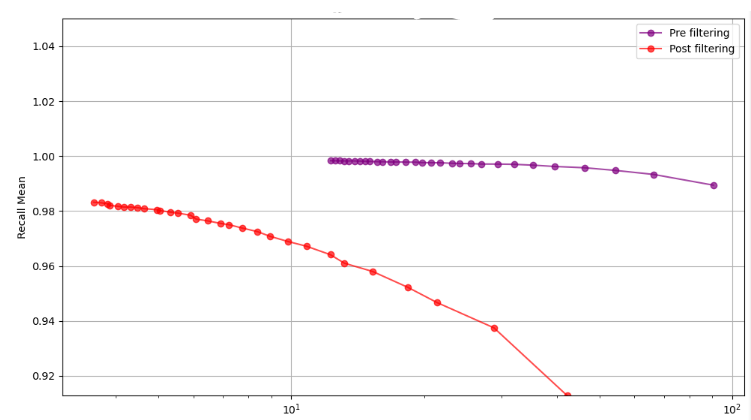
\includegraphics[width=0.4\textwidth]{IMAGES/immagine_2025-03-03_154956860.png}
    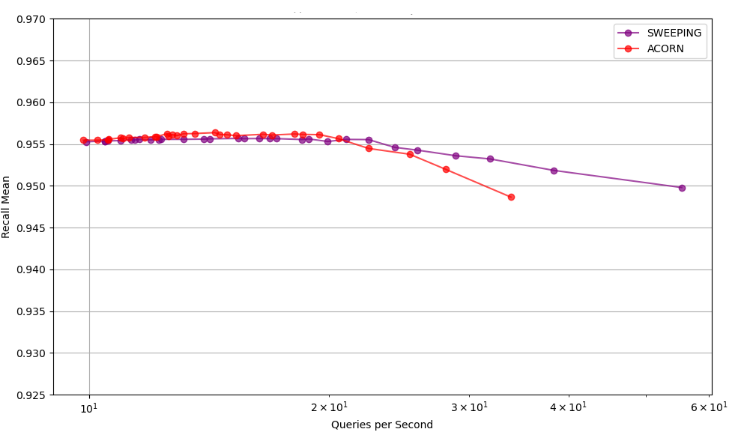
\includegraphics[width=0.4\textwidth]{IMAGES/immagine_2025-03-03_150720257.png}
    \caption{Performance comparison in Weaviate.}
    \label{fig:Weaviate}
\end{figure}
\section{Range Filtering ANN}
Range Filtering ANN (RFANN) is used for high-dimensional data where each vector has an associated, ordered attribute. Given a dataset \( D \), a query vector \( q \), a parameter \( K \), and a query range \([x, y]\), RFANN aims to find the approximate \( K \) nearest upper neighbors in \( D \) whose attributes fall within \([x, y]\). This is valuable in applications like e-commerce, where users filter products by price. However, such searches can be computationally expensive. Common approaches—Post-Filtering, In-Filtering, and Pre-Filtering—each have limitations: Post- and In-Filtering struggle with high-selectivity queries, while Pre-Filtering becomes inefficient with large datasets. Optimizing resource usage and performance remains a key challenge.


\section{Naive Solution}
A simple but impractical approach to solving range-filtering approximate nearest neighbor (RFANN) queries is to build dedicated graph-based indexes for all possible query ranges. However, this does not scale well. Given a collection of $n$ objects, the number of possible query ranges grows to $O(n^2)$. 

\section{IRangeFiltering}
IRangeGraph is a novel method designed to handle range-filtering queries efficiently without constructing a massive number of dedicated indexes. Instead of materializing a separate graph for each query range, \textbf{IRangeGraph constructs a moderate number of precomputed graphs, called elemental graphs}, which are later used to dynamically build the required index for any given query range.

The key benefits of IRangeGraph are:
\begin{itemize}
    \item \textbf{On-the-fly graph construction}: Instead of storing all possible dedicated graphs, it dynamically assembles a graph from \textit{elemental graphs} corresponding to segments of the data.
    \item \textbf{Efficient querying}: Despite constructing the graph during query execution, the overhead is low, and performance is close to that of fully materialized dedicated graphs, while using significantly less memory.
\end{itemize}

\subsection{Constructing Elemental Graphs and Forming Dedicated Graphs}
To efficiently construct elemental graphs, \textbf{IRangeGraph leverages a segment tree}:
\begin{itemize}
    \item The segment tree has \textbf{$O(\log n)$ layers}, where each node represents a range of objects.
    \item The \textbf{root node} corresponds to the entire dataset.
    \item Each \textbf{child node} represents a sub-range, recursively partitioning the dataset into smaller segments.
    \item \textbf{Leaf nodes} correspond to individual objects (segments of size 1), meaning it contains elements with the same values.
    \item Each segment stores an \textbf{elemental graph}, which serves as a building block for constructing query-specific graphs \cite{irangegraph}.
\end{itemize}


Each \textbf{node} in the segment tree, not just the leaves, has its own elemental graph materialized. This means that an elemental graph is constructed for every segment at every level of the segment tree, leading to a total of $O(n \log n)$ elemental graphs across the entire structure \cite{irangegraph}.



\subsection{Dedicated Graph Construction}
In order to construct on-the-fly the dedicated graph, IRangeGraph utilizes the concept of the \textbf{Relative Neighborhood Graph (RNG)}. Which ensures that an edge between two objects exists only if no other object is significantly closer to both of them. This pruning rule helps maintain a sparse yet effective structure for nearest neighbor search. 

When a query is issued with a given range $[L, R]$, IRangeGraph constructs the required graph dynamically:
\begin{enumerate}
    \item Identify the \textbf{elemental graphs} that intersect with the query range.
    \item Combine relevant edges from these elemental graphs to form the dedicated graph.
    \item Apply \textbf{RNG pruning rules} to retain only essential edges.
\end{enumerate}


\subsubsection{Example: Querying a Specific Range}
Consider a dataset with values in the range $[0,4]$ and an issued query for the range $[2,3]$. The segment tree structure would include:
\begin{itemize}
    \item A root node covering the full range $[0,4]$.
    \item Child nodes covering $[0,2]$ and $[3,4]$.
    \item Further subdivisions where necessary, with leaf nodes at individual values.
\end{itemize}

\begin{figure}[h]
    \centering
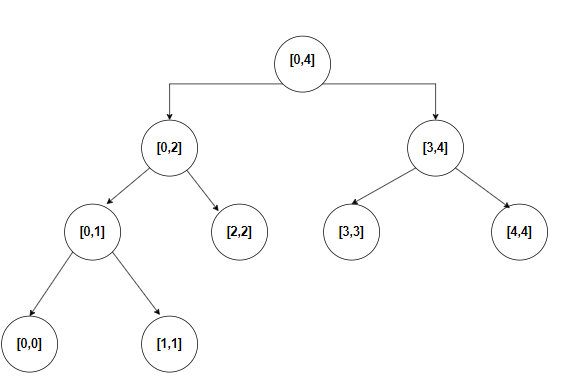
\includegraphics[width=0.8\textwidth]{IMAGES/immagine_2025-02-28_120223507.png}
    \caption{Example of Segment Tree.}
    \label{fig:Segment Tree}
\end{figure}

For the query $[2,3]$:
\begin{enumerate}
    \item The elemental graphs corresponding to segments $[2,2]$ and $[3,3]$ are selected since they fully intersect with the query range.
    \item Additionally, the segment $[2,3]$ is selected, as it directly encompasses the range.
    \item The relevant edges from these elemental graphs are combined to construct the dedicated graph.
    \item The resulting graph enables efficient nearest neighbor search within the range $[2,3]$.
\end{enumerate}

\section{Segment Graph for RFANN Search (SeRF)}
SeRF addresses the issue of the Naive approach by introducing a \textit{segment graph}, which losslessly compresses these $n$ HNSW indexes into a single structure with a significantly reduced memory footprint. The data structure is refereed as Segment Graph, which organizes the neighbor relationships dynamically across different ranges, permitting to represent the the connectivity of $n$ HNSW graphs using only $\mathcal{O}(nM)$ space, where $M$ is the maximum degree of nodes in HNSW.

This is achieved through:
\begin{itemize}
    \item Storing each edge only once, annotated with its active range $[b, e]$, instead of duplicating it across multiple graphs.
    \item Avoiding the explicit storage of $n$ independent HNSW graphs, leading to a compression factor of approximately $\mathcal{O}(n)$ in the worst case.
    \item Ensuring efficient query execution by enabling range-based edge retrievals without reconstructing multiple indexes.
\end{itemize}

\subsection{Segment Graph construction}
The construction follows these key steps:
\begin{enumerate}
    \item \textbf{Sequential HNSW Insertion:}  
    Data points are sorted based on their associated attribute values. The HNSW graph is incrementally built in an ordered manner, meaning that at step $x$, the index constructed so far contains only the first $x$ points.

    \item \textbf{Tracking Persistent Neighbor Relationships:}  
    When adding a new point $v_x$ to the graph, its approximate nearest neighbors are determined using an ANNS search over the existing structure. These neighbors are then pruned to ensure efficient navigation in the HNSW hierarchy. Instead of storing these neighbor connections separately for each step, we record their validity over a \textit{segment range} $[b, e]$, where:
    \begin{itemize}
        \item $b$ represents the insertion step when the edge was first added.
        \item $e$ represents the step at which the edge was removed due to the pruning process.
    \end{itemize}
    
    \item \textbf{Segment-Based Edge Storage:}  
    Each edge $(v_i, v_j)$ in the segment graph is stored as a tuple $(v_j, b, e)$ in the adjacency list of $v_i$. This means that $v_j$ remains a neighbor of $v_i$ in all query-specific graphs from step $b$ to $e$. Instead of storing $n$ redundant graphs, this method encodes all necessary information in a single compressed structure.

    \item \textbf{Edge Pruning and Updates:}  
    When a new node $v_x$ is inserted, it may cause the removal of certain edges due to dominance criteria in HNSW pruning (i.e., when a new node provides a more efficient navigation path). The segment graph updates the validity range of affected edges dynamically, ensuring that removed edges are correctly marked with an endpoint $e = x - 1$.
\end{enumerate}

\section{Further Compression of the Segment Graph}  
SeRF compresses multiple HNSW indexes into a single segment graph but is limited to static datasets. The \textbf{Dynamic Range-Filtering Approximate Nearest Neighbor Search (DRFANN)} model enhances adaptability with a \textit{dynamic segment graph}, enabling incremental updates while reducing redundancy and storage overhead.  

By integrating a rectangle tree and dynamic segment graph, DRFANN surpasses static RFANN methods (SeRF, iRangeGraph, etc.):  
\begin{itemize}  
    \item \textbf{Supports Dynamic Data:} Allows unordered vector insertions.  
    \item \textbf{Compact Indexing:} Reduces $\mathcal{O}(n^2)$ HNSW graphs to $\mathcal{O}(n \log n)$ edges.  
    \item \textbf{Efficient Queries:} Eliminates costly ANN result merging.  
    \item \textbf{Fast Updates:} Only $\mathcal{O}(\log n)$ edges are modified per insertion.  
\end{itemize}  

\subsection{Dynamic Segment Graph and Compression}  
The \textbf{dynamic segment graph} represents RFANN query ranges in a single, continuously updated structure. Instead of duplicating HNSW graphs, it assigns each edge a rectangular validity label $(l, r] \times [b, e)$, indicating the attribute range where the edge remains valid.  

\subsection{Graph Construction}  
As new vectors arrive, the dynamic segment graph is updated as follows:  
\begin{enumerate}  
    \item \textbf{Rectangle Representation:} Each edge $(v_i, v_j)$ is assigned a validity range $(l, r] \times [b, e)$.  
    \item \textbf{Edge Reuse:} Edges are shared across overlapping query ranges, minimizing storage.  
    \item \textbf{Incremental Updates:} New insertions adjust only $\mathcal{O}(\log n)$ edges, preventing index bloat.  
\end{enumerate}  




\subsection{Rectangle Tree for Space Partitioning}  
The \textit{rectangle tree} hierarchically partitions query ranges, optimizing storage and retrieval:  
\begin{itemize}  
    \item Inserting a vector with attribute \textbf{x} initializes a root node covering $(-\infty, x] \times [x, \infty)$.  
    \item Nearest neighbors are retrieved iteratively, with layer $n$ containing $n$ shared neighbors.  
    \item Nodes represent query ranges $(l, r] \times [b, e]$, reducing redundancy.  
    \item Leaf nodes store approximate nearest neighbors (ANNs) for fast lookup.  
    \item Internal nodes partition the search space, ensuring efficient range-filtered searches.  
\end{itemize}  


\subsection{Example of Insertion in Dynamic Segment Graph}
To better understand the how the Dynamic Segment Graph works, we illustrate the process of the insertion of a new vector. Let the existing dataset consist of nine vectors, each with an associated attribute value, and suppose we insert a new vector:
\[
v10 \quad \text{with attribute value } 54.
\]


\begin{table}[h]
    \centering
    \begin{tabular}{c|c|c}
        \hline
        \textbf{Vector} & \textbf{Distance to $v_{10}$} & \textbf{Attribute} \\
        \hline
        $v_1$ & 2  & 28  \\
        $v_2$ & 18 & 36  \\
        $v_3$ & 17 & 68  \\
        $v_4$ & 8  & 37  \\
        $v_5$ & 4  & 43  \\
        $v_6$ & 11 & 56  \\
        $v_7$ & 9  & 57  \\
        $v_8$ & 13 & 66  \\
        $v_9$ & 10 & 35  \\
        \hline
    \end{tabular}
    \caption{Dataset before inserting $v_{10}$.}
\end{table}


\begin{enumerate}  
    \item Identify the $K$ nearest neighbors using the existing segment graph.  
    \item Initialize an R-tree with root $(-\infty, 54] \times [54, \infty)$, representing $v_{10}$'s rectangle.  
    \item Partition the range space iteratively using the $K$ nearest neighbors.  
    \item Update the \textbf{rectangle tree} to incorporate the new attribute ranges.  
    \item Add edges upon reaching the child nodes.  
\end{enumerate} 



\begin{figure}[h]
    \centering
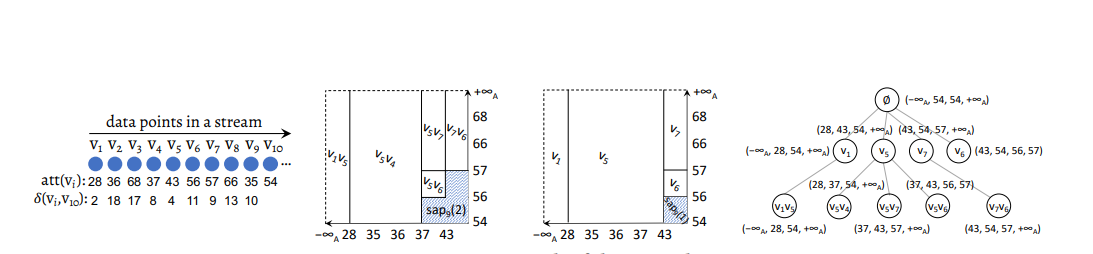
\includegraphics[width=1.1\textwidth]{IMAGES/immagine_2025-03-01_191002770.png}
    \caption[Rectangle Tree]{Rectangle Tree and range space partitioning. Source: Miaoqiao\footnotemark[2]}
    \label{fig:Rectangle Tree}
\end{figure}
\footnotetext[2]{\url{https://miaoqiao.github.io/paper/VLDB25_TR.pdf}}

% CHAPTER 6
\pagestyle{fancy}
\chapter{RAG}  
\label{chap:RAG}  
This chapter explores Retrieval-Augmented Generation (RAG), which enhances Large Language Models (LLMs) by integrating retrieval from Vector Databases (VDBMSs) to mitigate their limitations. We discuss alternative RAG approaches, including Agentic RAG, which leverages AI agents for iterative reasoning and refinement.


\section{Retrieval-Augmented Generation}  
Large Language Models (LLMs) are trained on vast datasets, but they face challenges when queried about information beyond their training data. In such cases, they may either admit a lack of knowledge or, worse, generate inaccurate responses—a phenomenon known as hallucination. 

LLMs, despite their capabilities, have two significant limitations:  
\begin{itemize}  
    \item They can confidently produce incorrect or outdated information (hallucinations).  
    \item They may not have been trained on the specific data required for a given query.  
\end{itemize}  


Retrieval-Augmented Generation (RAG) addresses this issue by supplementing LLMs with relevant external data. Instead of relying solely on pre-trained knowledge, RAG retrieves pertinent documents and incorporates them into the prompt, ensuring more accurate and context-aware responses. This approach is sometimes referred to as generative search or in-context learning.  

RAG mitigates these issues through a two-step process:  
\begin{enumerate}  
    \item \textbf{Retrieval} – Relevant information is fetched based on a query.  
    \item \textbf{Generation} – The LLM is then prompted with both the retrieved data and the user's query, allowing it to generate a response using up-to-date and relevant information.  
\end{enumerate}  

By leveraging retrieval-based augmentation, RAG enhances the accuracy and reliability of LLM outputs, reducing reliance on potentially outdated or incorrect pre-trained knowledge.



\section{Agentic Retrieval-Augmented Generation (RAG)}

Retrieval-Augmented Generation (RAG) enhances Large Language Models (LLMs) by incorporating external knowledge, improving accuracy, and reducing hallucinations. Instead of relying solely on the static knowledge encoded during pretraining, RAG retrieves relevant information from external sources to provide more accurate, up-to-date, and contextually appropriate responses. 

However, traditional RAG approaches have several limitations:

\begin{itemize}
    \item \textbf{Static retrieval and generation process:} The retrieval step typically happens only once before the generation phase, which means there is no opportunity for iterative refinement based on context or response quality.
    \item \textbf{Limited to a single external knowledge source:} Most RAG implementations retrieve information from a single vector database (VDB), but some use cases require multiple sources, such as APIs, structured databases, or web-based knowledge repositories.
    \item \textbf{Lack of reasoning over retrieved information:} The retrieved context is used as-is without further validation, filtering, or iterative reasoning, potentially leading to the propagation of incorrect or incomplete information.
\end{itemize}

\subsection{Introducing Agentic RAG}
Agentic RAG extends the traditional RAG paradigm by introducing AI agents—autonomous LLM-based systems that perform specialized tasks while leveraging dynamic retrieval, reasoning, and tool use. Unlike standard RAG, which retrieves and applies context in a single step, agentic systems operate iteratively, refining their approach and responses through multiple retrieval and reasoning cycles.

In an agentic framework, each agent has a specific role, allowing for modular execution where tasks are divided and optimized at different stages. The agents operate in a structured, step-by-step manner, where each stage builds upon previous results, ensuring continuous improvement in response quality.

The key components of an AI agent include:

\begin{itemize}
    \item \textbf{LLM:} The core reasoning and generation engine responsible for processing information and making decisions.
    \item \textbf{Task:} A predefined objective or role assigned to the agent, guiding its execution strategy.
    \item \textbf{Long-term memory:} A persistent storage system, often implemented using vector databases (VDBMs), enabling the agent to retain learned information over multiple interactions.
    \item \textbf{Short-term memory:} A temporary state tracker that maintains context throughout execution, enabling dynamic workflow adjustments and information flow between agent interactions.
    \item \textbf{Tools:} External utilities such as APIs, databases, search engines, code execution environments, or computational functions that extend the agent's capabilities beyond text-based generation.
\end{itemize}

By leveraging these components, agents can actively retrieve, analyze, and refine information rather than passively relying on a single retrieval step. This iterative approach results in more contextually accurate and reliable responses.

\subsection{Agentic RAG and Agent-Based Frameworks}

Agentic RAG integrates agent-based frameworks with RAG, creating a dynamic pipeline that iteratively retrieves, reasons, and refines information. This approach addresses the limitations of static retrieval by enabling LLMs to interact with external tools, break down complex tasks, and continuously adapt based on intermediate results.

Unlike traditional RAG, which retrieves data once and directly uses it for generation, Agentic RAG incorporates multiple retrieval cycles, validation mechanisms, and step-by-step task execution. The agent can refine the retrieved information, cross-check responses, and adapt its approach dynamically.

Key characteristics of Agentic RAG include:

\begin{itemize}
    \item \textbf{Autonomous execution:} Agents execute tasks independently, continuously assessing and refining their output based on intermediate feedback.
    \item \textbf{Multi-step decision-making:} Instead of retrieving information once, agents can perform multiple queries, validate responses, apply logical reasoning, and adjust their strategy as needed.
    \item \textbf{Tool integration:} Agents leverage APIs, databases, and computational tools to dynamically fetch, analyze, and process external data beyond what is stored in their training corpus.
    \item \textbf{Dynamic adaptation:} Agents can modify their retrieval strategy based on contextual cues, ensuring more relevant and precise results.
    \item \textbf{Progressive refinement:} The agent iteratively improves responses by retrieving additional data, analyzing inconsistencies, and updating its understanding.
\end{itemize}

\section{Agentic Frameworks}

Agentic frameworks provide structured methodologies for developing AI agents that integrate reasoning, retrieval, and action execution. These frameworks enable the creation of more intelligent and autonomous LLM-powered systems by allowing agents to dynamically interact with tools, retrieve external knowledge, and refine their responses iteratively. By leveraging these frameworks, developers can design AI agents that retrieve information more accurately, adapt dynamically to new inputs, and maintain context over extended interactions.


\subsection{ReAct Framework}

One widely adopted framework for agent-based reasoning is the ReAct framework, which stands for \textbf{Reason + Act}. A ReAct agent processes sequential, multi-step queries while maintaining state by combining reasoning, tool use, and query planning into a cohesive workflow.

The ReAct process follows an iterative cycle:

\begin{itemize}
    \item \textbf{Thought:} Upon receiving a query, the agent reasons about the next action.
    \item \textbf{Action:} The agent executes the decided action, such as querying a database, calling an API, or retrieving relevant documents.
    \item \textbf{Observation:} The agent evaluates the output of the action and determines the next step.
\end{itemize}

This cycle repeats until the agent reaches a final response. The iterative nature of ReAct allows it to refine answers dynamically, validate retrieved information, and adjust its approach based on real-time observations.

\subsection{LangChain and LangGraph}

Several frameworks have emerged to facilitate the development of agentic systems, with \textbf{LangChain} and \textbf{LangGraph} being two of the most prominent. While both are designed to enable LLM-powered applications, they differ in their execution models and capabilities.

\subsubsection{LangChain: Modular and Sequential Execution}

LangChain provides a modular architecture for integrating LLMs with various external tools, databases, and APIs. It offers structured workflows for chaining multiple components, such as prompt templates, memory modules, and tool interfaces.

Key characteristics of LangChain:
\begin{itemize}
    \item \textbf{Sequential Execution:} LangChain primarily follows a linear pipeline, where tasks are executed in a predefined order.
    \item \textbf{Memory Management:} It supports both short-term and long-term memory, enabling persistent context handling across interactions.
    \item \textbf{Tool Integration:} LangChain allows agents to interact with APIs, databases, and custom functions, expanding their ability to fetch and process information.
    \item \textbf{Pre-built Components:} Developers can leverage pre-configured templates for common use cases, simplifying implementation.
\end{itemize}

LangChain is well-suited for structured LLM applications, such as chatbots, document retrieval systems, and structured automation pipelines, where execution follows a predictable sequence.

\subsubsection{LangGraph: Graph-Based Execution for Agentic Systems}

LangGraph extends LangChain by introducing a \textbf{graph-based execution model}, allowing agents to perform dynamic, non-linear reasoning and iterative refinement. Unlike LangChain’s sequential structure, LangGraph enables flexible workflows where execution can be cyclic, conditional, or parallel.

Key differences of LangGraph:
\begin{itemize}
    \item \textbf{Graph-Based Workflow:} Instead of a linear pipeline, LangGraph represents tasks as nodes and execution logic as edges, enabling more complex task decomposition.
    \item \textbf{Cyclic Execution:} Supports iterative reasoning, allowing agents to refine responses through multiple retrieval and validation steps.
    \item \textbf{Conditional Logic:} Agents can make real-time decisions based on retrieved information, enabling adaptive responses.
    \item \textbf{Multi-Agent Coordination:} Facilitates communication between multiple agents, each specialized for different tasks, improving efficiency in complex workflows.
\end{itemize}

LangGraph is particularly useful for applications requiring multiple retrieval steps, adaptive decision-making, and real-time processing, such as dynamic research assistants, financial analysis bots, and multi-agent orchestration systems.

\subsection{Example of Document Retrieval with LangGraph}
As previously mentioned, Agentic RAG helps overcome the limitations of static RAG. One such improvement can be observed in the following experiment. The initial setup consists of a vector database containing PubMed documents indexed using an HNSW index. Each document includes a title, abstract, and tags, all of which are embedded using the multilingual Ollama model. The challenge arises during querying: when searching for documents related to \textit{breast cancer}, the vector database embeds the query, retrieves the top $K$ matching documents, and forwards them to the LLM for response generation. However, if an irrelevant but semantically similar document (such as documents about mouth cancer or cancer in general) is included in the retrieved set, the LLM may produce suboptimal results due to the presence of non-relevant context.

\begin{figure}[h]
    \centering
    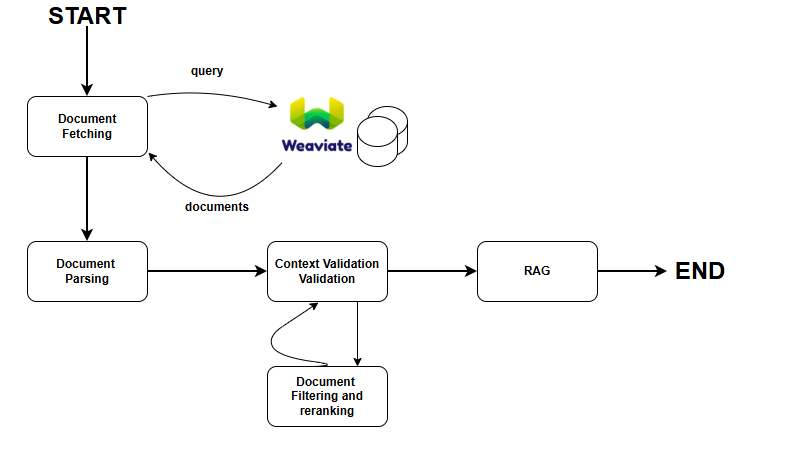
\includegraphics[width=0.8\textwidth]{IMAGES/immagine_2025-03-22_165130054.png}
    \caption[LangGraph Workflow]{LangGraph Workflow for Document Retrieval.}
\end{figure}


LangGraph addresses this issue by introducing a structured, step-by-step retrieval process where each agent performs a distinct task. These tasks include:
\begin{itemize}
    \item Fetching documents from the vector store
    \item Parsing the vector database output
    \item Validating the retrieved context using an LLM
    \item Correcting and re-ranking the context
    \item Providing the refined context to the LLM
\end{itemize}
This structured approach significantly enhances the RAG workflow by ensuring more accurate results while also standardizing the retrieval process.

\chapter{GraphRAG}
This chapter introduces the concept of Retrieval-Augmented Generation (RAG) in conjunction with Knowledge Graphs, which serve as structured data representations that capture complex relationships between entities. Knowledge Graphs are particularly advantageous due to their ability to synthesize information and reveal intricate connections between data points, making them an effective tool for enhancing retrieval-based AI models. We begin by exploring the applications of Graph RAG, demonstrating how it improves information retrieval by leveraging structured data. Following this, we delve into the core experiment of this thesis: the implementation of an Agentic RAG system that utilizes a Knowledge Graph to represent relational database schemas. This innovative approach enables efficient graph traversal for SQL query generation, enhancing both the explainability and accuracy of the generated queries.

\section{Knowledge Graphs and GraphRAG}
Another RAG approach that has been lately gaining traction employs the graph based data structures known as Knowledge Graphs. These structures are particularly useful for representing entities as nodes and the relationships between them with edges.
\begin{figure}[h]
    \centering
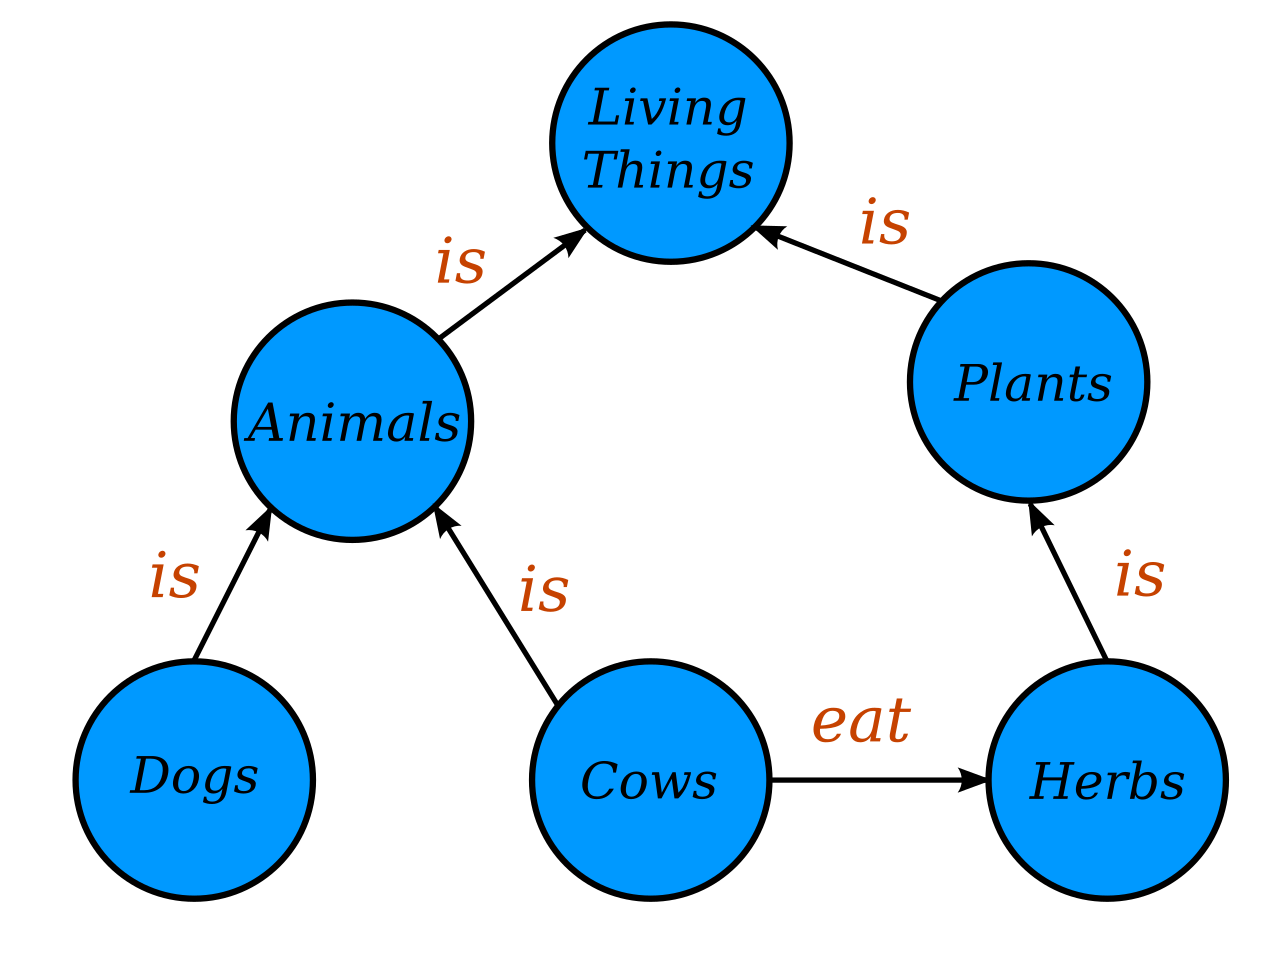
\includegraphics[width=0.65\textwidth]{IMAGES/Conceptual_Diagram_-_Example.svg.png}
    \caption[Knowledge Graph]{Example of Knowledge Graph. Source: Wikipedia\footnotemark}
    \label{fig:Knowledge Graph}
\end{figure}
\footnotetext{\url{https://en.wikipedia.org/wiki/Knowledge_graph}}
These graphs are widely used in AI-driven applications to enhance contextual understanding and reasoning by encoding explicit relationships between concepts. By structuring information in this way, knowledge graphs enable more sophisticated retrieval mechanisms beyond simple keyword or embedding-based searches. 

\subsection{GraphRAG: A Knowledge Graph-Driven RAG Approach}
In the context of Retrieval-Augmented Generation (RAG), knowledge graphs provide an alternative to traditional vector-based retrieval by making us of the more meaningful connections between concepts. While Vector based RAG systems rely on dense vector embeddings to find semantically similar text snippets, while being an effective technique is struggles with the sense making tasks that require understanding the relationships between entities across an entire dataset.

\subsection{Key Differences Between GraphRAG and Vector RAG}
The primary distinction between GraphRAG and Vector RAG lies in their retrieval mechanisms and capacity for global reasoning:

\begin{itemize}
    \item 	\textbf{Retrieval Mechanism:} Vector RAG uses embedding similarity to find relevant item, whereas GraphRAG navigates structured relationships within a knowledge graph.
    \item 	\textbf{Sensemaking Ability:} GraphRAG excels at answering global questions that require synthesizing information across multiple documents, while Vector RAG is better suited for fact-based, localized retrieval.
    \item 	\textbf{Scalability and Efficiency:} While GraphRAG requires an initial indexing phase to construct the knowledge graph, it can efficiently retrieve high-quality summaries for complex queries without retrieving an excessive number of items.
\end{itemize}


\subsection{Examples of Graph RAG  applications with LangChain}

With LangChain, we can provide a robust framework for integrating LLMs with our graph database by dynamically generating Cypher queries based on user questions. LangChain promotes seamless interaction between LLMs and graphs through the following components:

\begin{itemize}
    \item \textbf{Graph Database:} A structured representation of knowledge, such as Neo4j, where entities and relationships are stored.
    \item \textbf{Prompt Engineering:} A carefully crafted prompt template to guide the LLM in generating precise Cypher queries.
    \item \textbf{Query Execution:} The generated Cypher query is executed against the Knowledge Graph to retrieve relevant information.
    \item \textbf{Response Synthesis:} The retrieved data is processed and formatted into a natural language response by the LLM.
\end{itemize}

\begin{figure}[h]
    \centering
    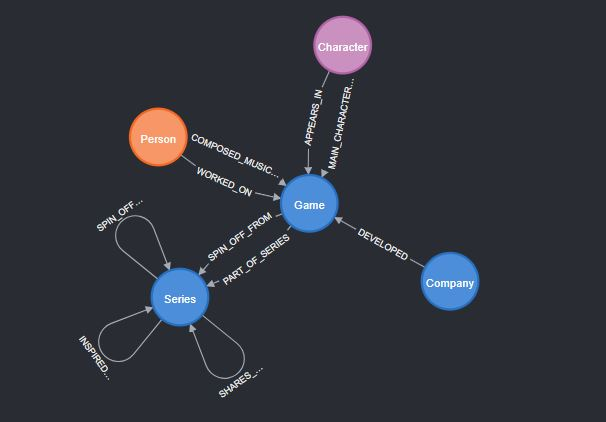
\includegraphics[width=0.9\textwidth]{IMAGES/Schema.JPG}
    \caption{KG schema visualized with APOC}
    \label{fig:Matching Nodes}
\end{figure}

In the figure above, we present a schema of our graph, which describes the entities related to game companies, the series produced, the people involved in game development, and even the characters. This serves as a heterogeneous knowledge base containing different types of entities connected to one another. 

For example, we can ask the LLM, \textit{"Which games has Kazuma Kaneko worked on?"} The chain responds with: \textit{"Kazuma Kaneko worked on Shin Megami Tensei III: Nocturne, Shin Megami Tensei V."} 


In the figure below, we illustrate the steps taken by LangChain:
\begin{figure}[h]
    \centering
    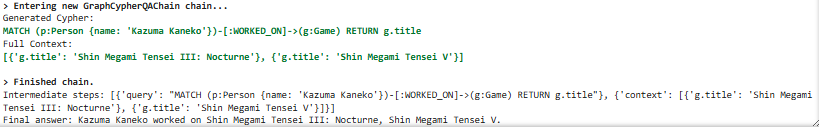
\includegraphics[width=1.1\textwidth]{IMAGES/immagine_2025-03-31_122504590.png}
    \caption{LangChain steps}
    \label{fig:Matching Nodes}
\end{figure}

Another angle worth exploring is the one about processing unstructured data into a Knowledge Graph. This way we can get the advantages of structured data such as finding complex relationships and patterns between entities, by starting from just a corpus of unstructured data. To construct this Knowledge Graph, LangChain leverages the use of an LLM that parses the text and categorizes the entities and their relationships. In the images below we can see the text corpus and the resulting schema of our generated Knowledge Graph.
\begin{figure}[h]
    \centering
    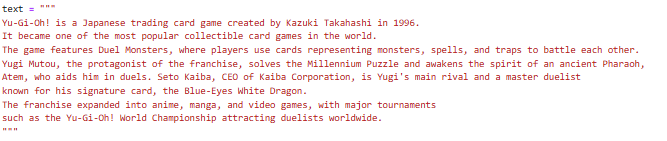
\includegraphics[width=1.1\textwidth]{IMAGES/immagine_2025-03-31_164059272.png}
    \caption{Text corpus}
    \label{fig:Matching Nodes}
\end{figure}
\begin{figure}[h]
    \centering
    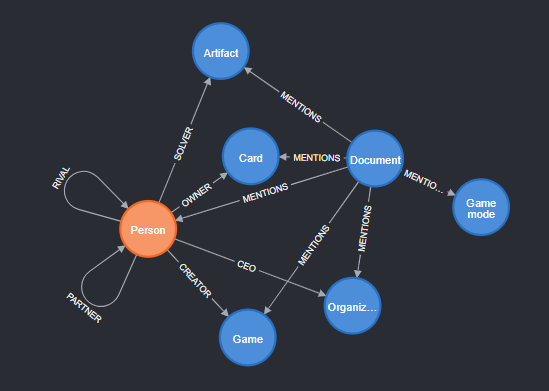
\includegraphics[width=0.7\textwidth]{IMAGES/immagine_2025-03-31_163821435.png}
    \caption{Generated Knowledge Graph}
    \label{fig:Matching Nodes}
\end{figure}


As demonstrated, LangChain effectively generates precise Cypher queries and retrieves relevant context from the Knowledge Graph to construct accurate responses. It is capable also of constructing Knowledge Graphs from unstructured data such as documents or corpus of text. However, while this approach is beneficial, it has limitations in handling more complex queries, and the still experimental nature of graph building dedicated LLMs, make it less suitable for production environments. A more adaptable solution for implementing Graph RAG is to utilize LangGraph, which enables greater control over workflow execution and allows for the incorporation of additional steps to improve response accuracy and handling of intricate queries.


\section{Experimental SQL generation with Knowledge Graphs}
In this final section, we present an experiment that integrates the theoretical principles discussed throughout this thesis. The experiment explores the use of Knowledge Graphs in generating SQL queries from natural language prompts. The workflow is built around LangGraph, which systematically processes natural language input to generate SQL queries. The process begins by constructing a Knowledge Graph from the schema of two CSV tables retrieved from the OpenData platform, which we will discuss shortly. This schema is represented as a Knowledge Graph in Neo4j, providing a structured understanding of the data relationships. LangGraph leverages a Large Language Model (LLM) to generate a Cypher traversal query, establishing connections between the two tables. The generated query then undergoes validation, ensuring it meets syntax requirements and other adequacy criteria before final execution.
\subsection{Workflow}

The general workflow of the architecture follows these steps:

\begin{enumerate}
    \item \textbf{Schema Analysis and Knowledge Graph (KG) Building}:  
    The CSV files are loaded, and a knowledge graph is constructed to represent the schema of the tables.

    \item \textbf{Vectorization and Storage}:  
    Column labels are vectorized and stored in a vector database, such as Weaviate, using Ollama.

    \item \textbf{Entity Matching}:  
    A two-step matching process is performed:  
    \begin{itemize}
        \item \textit{Label-Based Search}: Using cosine similarity to find relevant columns.  
        \item \textit{Value-Based Matching}: A customized scoring function evaluates whether columns can be joined based on their values.
    \end{itemize}

    \item \textbf{Schema Filtering}:  
    To improve Cypher query generation accuracy, schema elements irrelevant to the natural language question are filtered out. Only tables and relationships that exceed a predefined threshold are retained.

    \item \textbf{Question Enrichment}:  
    The natural language question is enriched with schema labels, reducing ambiguity and improving the mapping between the question and the schema for Cypher query generation.

    \item \textbf{Cypher Query Generation}:  
    A Cypher query is generated based on the enriched question and filtered schema.

    \item \textbf{SQL Generation}:  
    Finally, an SQL query is generated from the Cypher query.
\end{enumerate}


\subsection{Motivations}
Our experiment addresses the challenge of querying structured databases using natural language. Traditional database queries require structured syntax, such as SQL, which must adhere to the database schema and its constraints. However, users may not have full knowledge of the database structure—only a general understanding of the domain. Even with SQL expertise, writing accurate queries can be time-consuming and costly.  

To overcome these limitations, we propose a scalable framework that enables users to query databases using natural language while maintaining accuracy comparable to that of a data expert. This approach simplifies database interactions, reduces the need for deep schema knowledge, and enhances efficiency.

\subsection{Knowledge Graph Construction}
The \textbf{Knowledge Graph} serves as a structured data representation that captures entities and their relationships. The first step in the process is constructing the Knowledge Graph, where \textbf{tables and columns} are represented as \textbf{nodes}, and their relationships are defined by \textbf{edges}. Specifically, edges emphasize the association between columns and the tables they belong to.  

Additionally, column nodes include metadata such as:  
\begin{itemize}
    \item \textbf{Uniqueness} – to determine whether a column serves as an identifier.
    \item \textbf{Data type} – to ensure strict matching between columns of the same type, with the exception of cases where \textbf{float and integer} types may be considered compatible.
\end{itemize}

In the \textbf{Neo4j} graph, the possible relationships include:  
\begin{itemize}
    \item \textbf{"HAS COLUMN"} – an edge connecting a \textbf{table node} to its \textbf{column nodes}.
    \item \textbf{"SAME ATTRIBUTE"} – an edge linking \textbf{column nodes} that share the same label and metadata. However, if two columns match perfectly, instead of creating a relationship, they are \textbf{collapsed into a single node} to maintain data integrity.
\end{itemize}

By leveraging this \textbf{Knowledge Graph}, we enable traversals between columns that effectively represent \textbf{joins} between relational database tables.
\begin{figure}[h]
    \centering
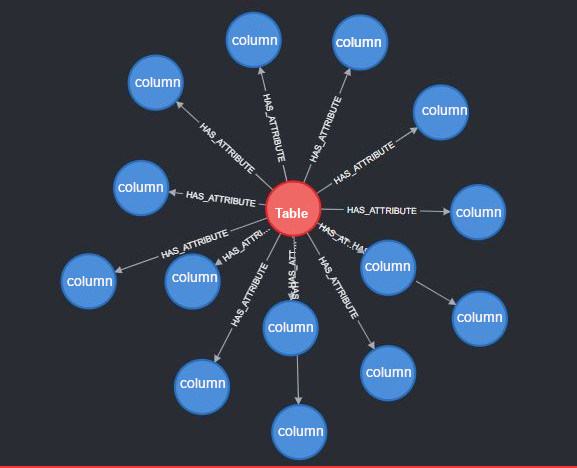
\includegraphics[width=0.7\textwidth]{IMAGES/KGschema.JPG}
    \caption{Example of generated Knowledge Graph}
    \label{fig:Knowledge Graph}
\end{figure}


\subsection{Entity Matching}
After constructing the Knowledge Graph, we also vectorize the column labels and store them in a Vector Database. For this, we use \textbf{Weaviate}, chosen for its lightweight processing, flexibility in vectorization, and ease of integration across platforms—thanks to its official \textbf{Docker} container. Weaviate supports multiple vectorization methods, and for this use case, we employ an \textbf{Ollama} container running the \textbf{snowflake-arctic-embed2} model, which provides fast and efficient lightweight vectorization.
\begin{figure}[h]
    \centering
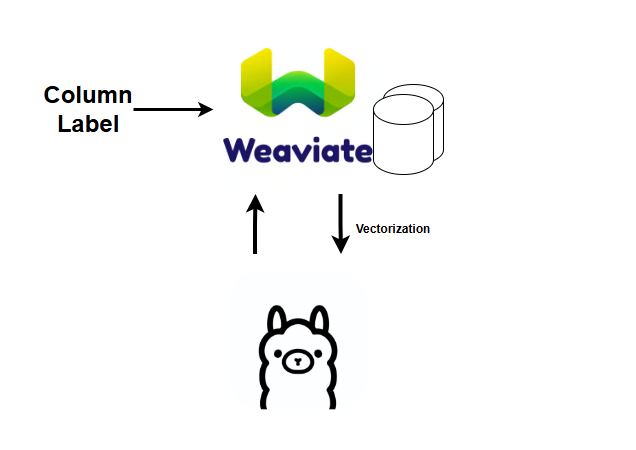
\includegraphics[width=0.65\textwidth]{IMAGES/immagine_2025-03-27_153710010.png}
    \caption{Column label vectorization}
    \label{fig:Vectorization}
\end{figure}
To store the vector embeddings, we use \textbf{Weaviate’s default flat index}, as the dataset contains only a few hundred embeddings. In this case, a flat search offers similar performance to \textbf{HNSW}, making it a practical choice for simplicity and efficiency.

Once the vector store is built, entity matching begins. Each column label undergoes a \textbf{vector search}, retrieving candidates with a similarity score above a predefined threshold. If a match meets this criterion, we perform a \textbf{value-based scoring} step to determine whether the columns are suitable for joining. A good join key should:

\begin{enumerate}
    \item \textbf{Have similar content} – The values should be closely related or directly matching.
    \item \textbf{Exhibit diversity} – Columns with excessive repetition (e.g., "Yes"/"No" or a single repeated category) provide little value in a join.
    \item \textbf{Share overlapping unique values} – Columns with entirely different value distributions are less useful for meaningful joins.
\end{enumerate}


The scoring process is based on a \textbf{TF-IDF vectorizer} provided by the \texttt{scikit-learn} library. The steps involved are as follows:

\begin{enumerate}
    \item The values within each column are vectorized using the TF-IDF method.
    \item A similarity matrix is computed, and the diagonal elements are extracted to calculate the mean similarity score.
    \item A penalty factor is applied to columns with a low diversity of unique values, reducing their overall score.
    \item The adjusted similarity score is compared against a predefined threshold to determine if the columns should be considered a match.
\end{enumerate}

If the similarity score exceeds the threshold, the Knowledge Graph is updated accordingly. The matched columns are linked via an edge labeled \textbf{"SAME ATTRIBUTE"}, which stores the computed similarity score as an edge property.
\begin{figure}[h]
    \centering
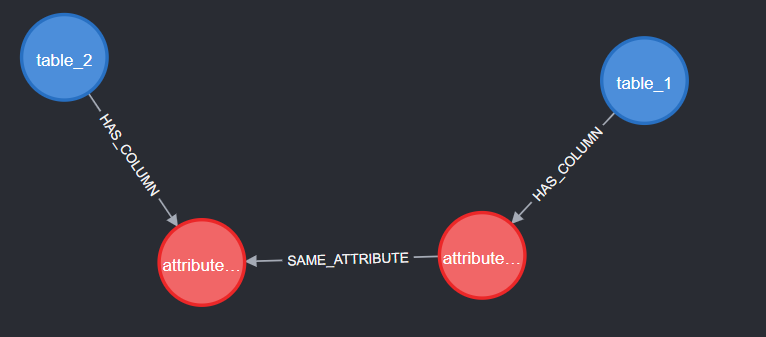
\includegraphics[width=0.7\textwidth]{IMAGES/immagine_2025-03-27_154727649.png}
    \caption{Example of matching nodes in the Knowledge Graph}
    \label{fig:Matching Nodes}
\end{figure}

\subsection{Schema Filtering and Question Enrichment}

After building the Knowledge Graph and Matching the entities, to enhance the accuracy of Cypher query generation, we introduce a two-step process: \textit{Schema Filtering} and \textit{Question Enrichment}.

\subsubsection{Schema Filtering}  
In this step, we refine the schema by filtering out elements that are not relevant to the given natural language question. Only tables and their traversals that meet a predefined relevance threshold are retained. This reduces noise and ensures that the generated Cypher query is based on the most pertinent schema components.The schema provides also similarity scores between nodes, this allows us to discern which column is needed to ensure the join statement.

\subsubsection{Question Enrichment}  
After schema filtering, the natural language question is enriched by incorporating schema labels and relationships between nodes. This step strengthens the connection between the question and the schema, reducing ambiguity and improving the precision of Cypher query generation. The expected resulting enriched prompt will contain the labels of the entities while still maintaining the sense of the original prompt.

\subsection{Cypher Generation with LangGraph Sub-Graphs}
For Cypher query generation, we leverage LangGraph's support for sub-graphs, enabling the construction of larger and more complex graphs in a modular manner. 
\begin{figure}[h]
    \centering
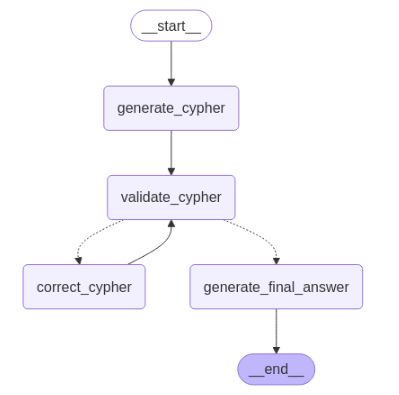
\includegraphics[width=0.55\textwidth]{IMAGES/LangGraph 2.JPG}
    \caption{Cypher Generation}
    \label{fig:Matching Nodes}
\end{figure}

The \textit{Cypher Generation} sub-graph begins with the provided enriched prompt and schema, generating the initial Cypher traversal. Once the traversal is created, an iterative process of validation and correction is employed to ensure the correctness of the query. 

To verify syntax accuracy, the query is executed using the \texttt{EXPLAIN} clause, which helps detect errors. Additionally, the process includes validating the existence of specific edges to ensure the correct generation of the Cypher query. Once validated, the final query is output to the main graph for further processing.


\subsection{SQL Translation from Cypher Traversal}

Once the Cypher query is generated, it provides a traversal that links table nodes through common neighbors, effectively representing the joining columns. This structured traversal serves as a bridge between the graph representation and relational databases, facilitating a seamless translation into SQL.

The SQL translation process closely mirrors the Cypher generation workflow, ensuring correctness through an iterative validation approach. Since the Cypher query already encodes the necessary relationships and joins, the translation primarily involves mapping graph-based traversals into equivalent SQL join operations. 

To guarantee syntactic accuracy, an iterative validation process is applied, similar to the validation performed during Cypher generation. This includes executing preliminary checks and leveraging SQL execution plans to detect potential syntax errors or logical inconsistencies. Any detected issues prompt refinements to the query before finalizing the SQL output. 

This structured approach ensures that the generated SQL query accurately reflects the intended data retrieval logic while maintaining correctness and efficiency.


\subsection{Execution over UK and Canadian OpenData}

After detailing the entire process, this section demonstrates its application to OpenData provided by Canada and the UK using SPARQL and CKAN. The UK dataset involves combining two CSV tables: one containing indicators of knee pain and the other related to varicose vein conditions. Once the Knowledge Graph (KG) is constructed, we observe that the provided code achieves the highest similarity score when joining tables within the filtered schema.

\paragraph{Nodes Representing Columns:}
\begin{itemize}
    \item \textbf{Procedure}  
        \begin{itemize}
            \item \texttt{data\_type}: string
            \item \texttt{is\_unique}: \texttt{False}
            \item \texttt{value}
            \item \texttt{similarity}: 0.9566
        \end{itemize}
    \item \textbf{Year}  
        \begin{itemize}
            \item \texttt{data\_type}: string
            \item \texttt{is\_unique}: \texttt{False}
            \item \texttt{value}
            \item \texttt{similarity}: 0
        \end{itemize}
    \item \textbf{AgeBand}  
        \begin{itemize}
            \item \texttt{data\_type}: string
            \item \texttt{is\_unique}: \texttt{False}
            \item \texttt{value}
            \item \texttt{similarity}: -2.6154
        \end{itemize}
    \item \textbf{ProviderCode}  
        \begin{itemize}
            \item \texttt{data\_type}: string
            \item \texttt{is\_unique}: \texttt{False}
            \item \texttt{value}
            \item \texttt{similarity}: 3.2149
        \end{itemize}
    \item \textbf{PostOpQReadmitted}  
        \begin{itemize}
            \item \texttt{data\_type}: int
            \item \texttt{is\_unique}: \texttt{False}
            \item \texttt{value}
            \item \texttt{similarity}: 1.9546
        \end{itemize}
    \item \textbf{VaricoseVeinPostOpQLeftFrontCount}  
        \begin{itemize}
            \item \texttt{data\_type}: int
            \item \texttt{is\_unique}: \texttt{False}
            \item \texttt{value}
        \end{itemize}
    \item \textbf{KneeReplacementPostOpQReadmitted}  
        \begin{itemize}
            \item \texttt{data\_type}: int
            \item \texttt{is\_unique}: \texttt{False}
            \item \texttt{value}
        \end{itemize}
    \item \textbf{KneeReplacementOKSPostOpQPredicted}  
        \begin{itemize}
            \item \texttt{data\_type}: float
            \item \texttt{is\_unique}: \texttt{False}
            \item \texttt{value}
        \end{itemize}
\end{itemize}
\linebreak 
\paragraph{Question Refinement:} \linebreak
\linebreak 
\linebreak  
Initially, the query posed was: 
\textit{"What is the average count of varicose vein post-op questions left front for knee replacement patients readmitted to hospital, by age band and provider code?"}  

The refined question, incorporating schema labels, is: \\ 
\textit{"What is the average \texttt{VaricoseVeinPostOpQLeftFrontCount} for \texttt{Procedure} 'Knee Replacement' patients with \texttt{PostOpQReadmitted} greater than 0, grouped by \texttt{AgeBand} and \texttt{ProviderCode}?"}  

This enrichment ensures greater specificity by aligning the query with structured schema elements.

\paragraph{Traversal and SQL Conversion:}
The Cypher traversal identifies the most optimal path between tables based on similarity scores, determining that the best route is through the \texttt{ProviderCode} node. 
The Cypher Traversal goes as follows:

\begin{figure}[h]
    \centering
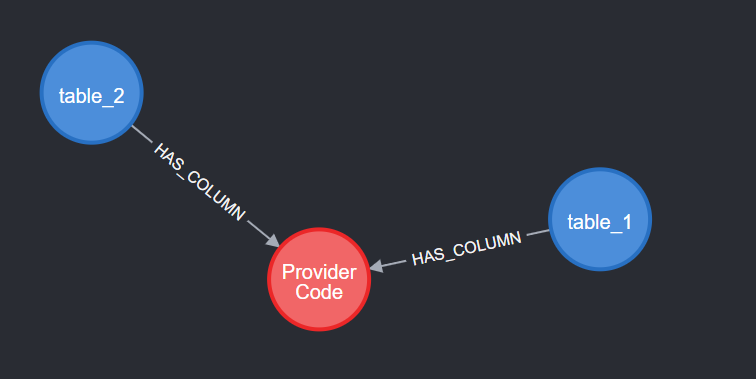
\includegraphics[width=0.65\textwidth]{IMAGES/immagine_2025-03-28_082503566.png}
    \caption{Generated Traversal}
    \label{fig:Traversal}
\end{figure}

This traversal is then converted into an equivalent SQL query:

\begin{verbatim}
SELECT T1.AgeBand, T1.ProviderCode, 
       AVG(T1.VaricoseVeinPostOpQLeftFrontCount) AS average_count
FROM Table1 T1
JOIN Table2 T2
ON T1.ProviderCode = T2.ProviderCode AND T1.AgeBand = T2.AgeBand
WHERE T2.PostOpQReadmitted IN (1, 'yes', TRUE, 'Yes') 
      AND T1.PostOpQReadmitted IN (1, 'yes', TRUE, 'Yes')
GROUP BY T1.AgeBand, T1.ProviderCode;
\end{verbatim}

\paragraph{Application to Canadian OpenData:}
For the query:  
\textit{"Get analysis types, values, and product types for Canadian samples"}  

The refined question becomes:  
\textit{"What are the \texttt{AnalysistypeTypedanalyse}, \texttt{ValuetextValeurtextuelle}, and \texttt{ProducttypeTypedeproduit} for samples from \texttt{CountryoforiginPaysdorigine} Canada?"}  

This results in the following SQL query:

\begin{verbatim}
SELECT DISTINCT 
    t1.AnalysistypeTypedanalyse AS analysis_type, 
    t1.ValuetextValeurtextuelle AS value, 
    t1.ProducttypeTypedeproduit AS product_type, 
    t2.AnalysistypeTypedanalyse AS analysis_type2, 
    t2.ValuetextValeurtextuelle AS value2, 
    t2.ProducttypeTypedeproduit AS product_type2
FROM Table1 t1
INNER JOIN Table2 t2 
ON t1.CountryoforiginPaysdorigine = t2.CountryoforiginPaysdorigine
WHERE LOWER(t1.CountryoforiginPaysdorigine) = LOWER('Canada') 
      AND LOWER(t2.CountryoforiginPaysdorigine) = LOWER('Canada');
\end{verbatim}

These examples illustrate how our methodology effectively refines user queries and generates precise SQL queries by leveraging Knowledge Graph-based enrichment.

\section{Join Discovery with a Knowledge Graph of \( N \) Tables}

Building upon the previously introduced job pipeline, we extend the process from joining two tables to handling a more complex use case involving \( N \) tables. The goal is to determine the necessary relational tables required for a given query. 
\subsection{Metadata Integration in the KG construction}
In this augmentation we keep the Knowledge Graph construction process mostly unchanged, aside from an additional step before the construction, which is fetching a sample of each CSV and instruct the LLM or a human operator to provide a brief description of what the relational table represents.This process is simple and straightforward making the difference between the performances of a human operator and a LLM minimal.
\begin{figure}[h]
    \centering
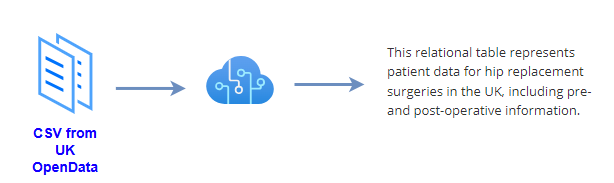
\includegraphics[width=0.65\textwidth]{IMAGES/immagine_2025-04-05_084400623.png}
    \caption{Example of an LLM's description of a Medical CSV}
    \label{fig:LLM CSV analysis}
\end{figure}


While the graph construction process remains almost unchanged, the primary modification occurs in the querying phase.
\subsection{Clustering in Knowledge Graph Representation}
As the Knowledge Graph representation grows in complexity, clustering becomes essential. This preliminary phase organizes the graph into clusters of \( N \) nodes, where each node represents a relational table. Nodes are connected if they share one or more common elements. 
\begin{figure}[h]
    \centering
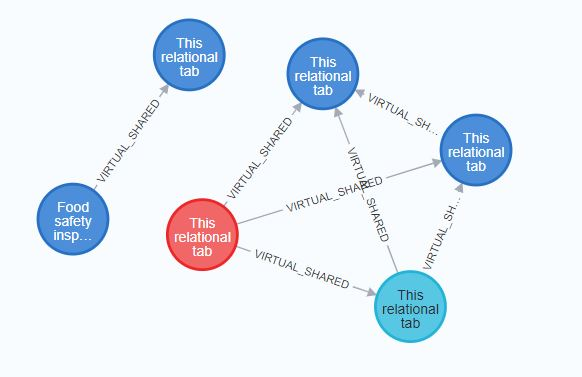
\includegraphics[width=0.65\textwidth]{IMAGES/Virtual Graph.JPG}
    \caption{Virtual Graph}
    \label{fig:Virtual Graph}
\end{figure}
By providing the LLM with the schema of the clustered Knowledge Graph, we can efficiently identify the most relevant nodes for a given query. This approach significantly reduces the graph’s size while maintaining performance comparable to the previous case involving only two tables. This approach allows for the system to scale very well as it greatly reduces the surface of the Knowledge Graph to explore, and can be stored in a persistence layer for later use, and gets reprocessed when a new CSV is fetched in our database still keeping a linear growth of complexity.

\section{Potential Improvements}

While the experiment establishes a standardized pipeline for generating structured SQL queries, several improvements can enhance its efficiency and adaptability:  

\begin{itemize}
    \item \textbf{Parallelization of LLM Prompting}: Implementing parallel processing can significantly speed up query generation by handling multiple prompts simultaneously.  
    \item \textbf{Federated Graph}: Using federated graph may allow to parallelize our system and scale it horizontally, with replication and also by keeping unrelated tables separated, removing unnecessary complexity from the workflow.
    \item \textbf{Automatic Language Detection}: Since the data sources primarily use English, querying non-English sources introduces additional complexity for the LLM in understanding both the prompt and schema. To address this, an automated language detection mechanism should be implemented. This process would:
    \begin{enumerate}
        \item Identify the language of the Open Data source.
        \item Translate the user prompt into the detected language.
        \item Generate the query in the appropriate language.
        \item Translate the final result back into the original language for consistency.
    \end{enumerate}
    \item  \textbf{Index vector store}: As the vector store increases in size the employment of specialized scalable indexes like HNSW may become more suitable, and it's worth to consider to use ACORN filtering strategy due to the correlation of the object and the querying predicate, also vector quantization may be useful in future uses.
    \item  \textbf{Automatically generated labels}: One challenge that must be tackled is the presence of automatically generated labels, which reduce significantly the sense making capabilities of the Knowledge Graph, for future applications this challenge is one of the main difficulties that must be dealt with. One possible approach is to employ an Hybrid matching between label and value based matching, between columns of matching data to improve robustness of the matching. Another possible approach is to employ a human operator to assess matching when the uncertainty is high during the matching task.
    \item \textbf{Security and query sanitation}: Security when it comes from fetching data from outside sources is always a concern to consider head on, API key must be stored in secure locations and not be put into the code or even an environment variable, if we're using containers the use of secrets is warranted. We make sure that the generated queries are sanitized and not executing an injection or other unauthorized operations. We analyze the data in order to assess that it's not tampered with, we validate and clean incoming data.
    \item \textbf{Keyword Extraction with CKAN Integration}: The system begins by extracting high-level keywords from the user’s natural language query. These keywords are used to query the CKAN open data portal via its API, leveraging available metadata for real-time dataset retrieval without prior ingestion or full indexing. If the initial keyword set is insufficient, the system iteratively refines the keywords to better match the query’s intent. Retrieved tables and metadata are stored in a structured dictionary for use in downstream processing.


\end{itemize}

These enhancements would improve both the performance and versatility of the system when handling diverse datasets.

\section{Conclusions}  

In this study, we explored the integration of Knowledge Graphs into Retrieval-Augmented Generation (RAG) to enhance the generation of SQL queries from natural language prompts. By leveraging structured relationships within a Knowledge Graph, GraphRAG provides a robust alternative to traditional vector-based retrieval methods, enabling more effective sensemaking and complex query generation. Unlike purely embedding-based retrieval approaches, which rely on semantic similarity and may struggle with structural dependencies, our framework introduces explicit relational reasoning, leading to more accurate and contextually relevant SQL query construction.  

Our experimental workflow demonstrated the feasibility of using LangGraph and Neo4j to systematically translate user queries into Cypher and SQL, ensuring both accuracy and efficiency. We implemented a hybrid retrieval strategy that combines entity matching through vector embeddings with value-based scoring, enabling more refined schema selection and join identification. This approach enhances the system’s ability to handle ambiguous or incomplete user queries by leveraging explicit graph relationships to infer missing connections. Furthermore, the multi-stage query refinement process allows for incremental improvements, ensuring that the generated SQL statements align closely with the intended query semantics.  

The evaluation of our framework over UK and Canadian OpenData datasets highlighted its effectiveness in translating natural language into precise SQL queries. We observed that the structured representation within the Knowledge Graph significantly improved the model’s ability to generate meaningful queries in complex database schemas, particularly in scenarios where conventional keyword-based retrieval failed to capture intricate table relationships. The introduction of Cypher-based retrieval prior to SQL generation facilitated improved schema sensemaking, reducing the occurrence of incorrect table joins and mismatched column references.  

While the current implementation effectively bridges natural language and structured data retrieval, several areas for future improvement remain. One key enhancement would be the parallelization of LLM prompting to reduce processing latency while maintaining high accuracy. Additionally, incorporating automatic language detection for multilingual query support could broaden the system’s applicability across diverse datasets. Further optimization of schema filtering techniques, including dynamic weighting of database elements based on query context, could further improve retrieval efficiency. Another promising avenue for exploration is the use of reinforcement learning or feedback-driven fine-tuning to iteratively enhance query generation based on user corrections and real-world usage patterns.  

Overall, this work contributes to the growing field of knowledge-driven query generation, demonstrating the potential of combining Knowledge Graphs and LLMs to simplify database interactions while maintaining expert-level accuracy. By integrating structured knowledge into the retrieval-augmented generation process, we enable more intelligent query formulation that extends beyond simple keyword matching. As AI-driven database querying continues to evolve, the fusion of structured and unstructured retrieval approaches, as demonstrated in this study, offers a promising path toward more intuitive and accessible data exploration tools.

% CHAPTER 7
%\input{BODY/7_CHAP/GRAPH_RAG}


% CONCLUSIONS
%% CONCLUSION FILE
\chapter*{Conclusions}
\addcontentsline{toc}{chapter}{Conclusions}\markboth{Conclusions}{}
\markboth{Conclusions}{Conclusions}
\lipsum[1-20]







% APPENDIX
%
% SETTING FOR APPENDIX ENVIRONMENT
{
\cleardoublepage
\let\clearpage\relax
\begin{LARGE}
\textbf{Appendix}
\end{LARGE}\\
\noappendicestocpagenum
\renewcommand{\appendixtocname}{Appendix}
\renewcommand{\appendixpagename}{Appendix}
\appendix
\addappheadtotoc
\chapter{Appendix title}
\label{appendix:first-appendix}
\normalsize
}
\lipsum[1-5]
% START APPENDIX
\section{First appendix section}
\lipsum[1-20]

\begin{thebibliography}{99}
\section*{References for Chapter 1}
\bibitem{deeplearning_vector_databases} DeepLearning.AI, \textit{Vector Databases and Embeddings Applications}, 2024. Available: \url{https://www.deeplearning.ai/short-courses/vector-databases-embeddings-applications/}.

\bibitem{deeplearning_retrieval_optimization} DeepLearning.AI, \textit{Retrieval Optimization: From Tokenization to Vector Quantization}, 2024. Available: \url{https://www.deeplearning.ai/short-courses/retrieval-optimization-from-tokenization-to-vector-quantization/}.

\bibitem{elastic_vector_embedding} Elastic, \textit{What is Vector Embedding?}, 2024. Available: \url{https://www.elastic.co/what-is/vector-embedding}.

\bibitem{pinecone_dense_vector_embeddings} Pinecone, \textit{Dense Vector Embeddings in NLP}, 2024. Available: \url{https://www.pinecone.io/learn/series/nlp/dense-vector-embeddings-nlp/}.

\bibitem{linkedin_encoding_vs_embedding} LinkedIn, \textit{Understanding Differences Between Encoding and Embedding}, 2024. Available: \url{https://www.linkedin.com/pulse/understanding-differences-between-encoding-embedding-mba-ms-phd/}.

\bibitem{levelup_vector_databases} LevelUp, \textit{6 Resources to Master Vector Databases and Building a Vector Storage}, 2024. Available: \url{https://levelup.gitconnected.com/6-resources-to-master-vector-databases-building-a-vector-storage-8d94ca1e3897}.

\bibitem{medium_vector_search} Tech Padawan Chronicles, \textit{Vector Search: Unlocking the Power of Unstructured Data}, 2024. Available: \url{https://medium.com/tech-padawan-chronicles/vector-search-unlocking-the-power-of-unstructured-data-ecf7c8ce91f6}.

\bibitem{ubiai_unstructured_data} UBIAI NLP, \textit{What is Unstructured Data? What Issues Can It Bring to Deep Learning Models in 2024?}, 2024. Available: \url{https://medium.com/ubiai-nlp/what-is-unstructured-data-what-issues-can-bring-to-the-deep-learning-model-in-2024-3410327dcc76}.


\section*{References for Chapter 2}


\bibitem{myscale_vector_indexing} MyScale, \textit{Understanding Vector Indexing: A Comprehensive Guide}, 2024. Available: \url{https://medium.com/@myscale/understanding-vector-indexing-a-comprehensive-guide-d1abe36ccd3c}.

\bibitem{freedium_neural_networks} Freedium, \textit{Overview of a Neural Network's Learning Process}, 2024. Available: \url{https://freedium.cfd/https://medium.com/data-science-365/overview-of-a-neural-networks-learning-process-61690a502fa}.

\bibitem{deeplearning_vector_databases} DeepLearning.AI, \textit{Vector Databases and Embeddings Applications}, 2024. Available: \url{https://www.deeplearning.ai/short-courses/vector-databases-embeddings-applications/}.

\bibitem{anishnama_encoder_decoder} Anish Nama, \textit{Exploring the Power of Encoder-Decoder Models: Pros, Cons, and Applications}, 2024. Available: \url{https://medium.com/@anishnama20/exploring-the-power-of-encoder-decoder-models-pros-cons-and-applications-8bfbe2e66e76}.

\bibitem{analyticsvidhya_neural_networks} Analytics Vidhya, \textit{Neural Networks in a Nutshell}, 2024. Available: \url{https://medium.com/analytics-vidhya/neural-networks-in-a-nutshell-bb013f40197d}.

\bibitem{builtin_transformer_nn} BuiltIn, \textit{Transformer Neural Network}, 2024. Available: \url{https://builtin.com/artificial-intelligence/transformer-neural-network}.

\bibitem{datacamp_vector_databases} DataCamp, \textit{The Top 5 Vector Databases}, 2024. Available: \url{https://www.datacamp.com/blog/the-top-5-vector-databases}.

\bibitem{schroff_facenet} Florian Schroff, Dmitry Kalenichenko, and James Philbin, \textit{FaceNet: A Unified Embedding for Face Recognition and Clustering}, in Proceedings of the IEEE Conference on Computer Vision and Pattern Recognition (CVPR), 2015. Available: \url{https://arxiv.org/abs/1503.03832}.

\bibitem{johnson_faiss} Jeff Johnson, Matthijs Douze, and Hervé Jégou, \textit{Billion-scale similarity search with GPUs}, arXiv preprint arXiv:1702.08734, 2017. Available: \url{https://arxiv.org/abs/1702.08734}.

\bibitem{mikolov_word2vec} Tomas Mikolov, Ilya Sutskever, Kai Chen, Greg S. Corrado, and Jeffrey Dean, \textit{Efficient Estimation of Word Representations in Vector Space}, arXiv preprint arXiv:1301.3781, 2013. Available: \url{https://arxiv.org/abs/1301.3781}.

    \bibitem{dlai} DeepLearning.ai, "Building Multimodal Search and RAG", \url{https://www.deeplearning.ai/short-courses/building-multimodal-search-and-rag/}.
    \bibitem{kxsystems} KX Systems, "Guide to Multimodal RAG for Images and Text", \url{https://medium.com/kx-systems/guide-to-multimodal-rag-for-images-and-text-10dab36e3117}.
    \bibitem{openai} OpenAI Cookbook, "Custom Image Embedding Search", \url{https://cookbook.openai.com/examples/custom_image_embedding_search}.
    \bibitem{langchain} Langchain Blog, "Semi-Structured Multi-Modal RAG", \url{https://blog.langchain.dev/semi-structured-multi-modal-rag/}.
    \bibitem{kinomoto} Kinomoto, "Convert Images to Embeddings for RAG", \url{https://medium.com/kinomoto-mag/convert-images-to-embeddings-for-rag-40447d16aaf2}.
    \bibitem{dataandbeyond} Data and Beyond, "Vector Databases: A Beginner's Guide", \url{https://medium.com/data-and-beyond/vector-databases-a-beginners-guide-b050cbbe9ca0}.
    \bibitem{arxiv} arXiv, "Understanding Multimodal Retrieval from an Embedding Perspective", \url{https://arxiv.org/abs/2310.14021}.




\section*{References for Chapter 3}

\bibitem{pinecone_pq} 
Pinecone. "Product Quantization."  
\url{https://www.pinecone.io/learn/series/faiss/product-quantization/}.

\bibitem{towards_datascience_pq} 
Towards Data Science. "Similarity Search & Product Quantization."  
\url{https://towardsdatascience.com/similarity-search-product-quantization-b2a1a6397701}.

\bibitem{deeplearning_ai_pq} 
DeepLearning.AI. "Retrieval Optimization: From Tokenization to Vector Quantization."  
\url{https://learn.deeplearning.ai/courses/retrieval-optimization-from-tokenization-to-vector-quantization/lesson/1/introduction}.

\bibitem{weaviate_pq} 
Weaviate. "Product Quantization in Vector Databases."  
\url{https://weaviate.io/developers/weaviate/concepts/vector-quantization#product-quantization}.

\bibitem{qdrant_pq} 
Qdrant. "Understanding Product Quantization."  
\url{https://qdrant.tech/articles/product-quantization/}.

\bibitem{weaviate_ann} 
Weaviate. "ANN Algorithms: Tiles Encoder."  
\url{https://weaviate.io/blog/ann-algorithms-tiles-enocoder}.

\bibitem{wikipedia_quantile} 
Wikipedia. "Quantile."  
\url{https://en.wikipedia.org/wiki/Quantile}.

\bibitem{wikipedia_cdf} 
Wikipedia. "Cumulative Distribution Function."  
\url{https://en.wikipedia.org/wiki/Cumulative_distribution_function}.

\bibitem{timescale_hnsw_vs_diskann} 
Timescale. "HNSW vs. DiskANN: A Comparison."  
\url{https://www.timescale.com/learn/hnsw-vs-diskann}.

\bibitem{milvus_diskann} 
Milvus. "DiskANN: An Efficient ANN Index."  
\url{https://milvus.io/blog/2021-09-24-diskann.md}.


\section*{References for Chapter 4}
\bibitem{vecindexing_myscale} 
Myscale Team. "Understanding Vector Indexing: A Comprehensive Guide." Medium, 2023. \url{https://medium.com/@myscale/understanding-vector-indexing-a-comprehensive-guide-d1abe36ccd3c}

\bibitem{oracle_hnsw} 
Oracle. "Understanding Hierarchical Navigable Small World Indexes." Oracle Database 23c Documentation. \url{https://docs.oracle.com/en/database/oracle/oracle-database/23/vecse/understand-hierarchical-navigable-small-world-indexes.html}

\bibitem{weaviate_flat} 
Weaviate. "Flat Vector Index." \url{https://weaviate.io/developers/academy/py/vector_index/flat}

\bibitem{pinecone_faiss} 
Pinecone. "Vector Indexes." \url{https://www.pinecone.io/learn/series/faiss/vector-indexes/}

\bibitem{mehta_vector_dbs} 
G. Mehta. "Understanding Vector DBs Indexing Algorithms." Medium, 2023. \url{https://gagan-mehta.medium.com/understanding-vector-dbs-indexing-algorithms-ce187dca69c2}

\bibitem{kdb_indexing} 
KDB.ai. "Indexing Basics." \url{https://kdb.ai/learning-hub/articles/indexing-basics/}

\bibitem{pinecone_lsh} 
Pinecone. "Locality-Sensitive Hashing (LSH)." \url{https://www.pinecone.io/learn/series/faiss/locality-sensitive-hashing/}

\bibitem{lsh_random_proj} 
Pinecone. "Locality-Sensitive Hashing Using Random Projection." \url{https://www.pinecone.io/learn/series/faiss/locality-sensitive-hashing-random-project}

\bibitem{lsh_querying} 
D. Turnbull. "Implementing Random Projections." SoftwareDoug, 2023. \url{https://softwaredoug.com/blog/2023/08/21/implementing-random-projections}

\bibitem{ivf_index} 
S. Jain. "Similarity Search: kNN & Inverted File Index." Towards Data Science, 2023. \url{https://towardsdatascience.com/similarity-search-knn-inverted-file-index-7cab80cc0e79}

\bibitem{faiss_vs_lsh} 
Facebook Research. "Comparison with LSH." FAISS Wiki. \url{https://github.com/facebookresearch/faiss/wiki/Comparison-with-LSH}

\bibitem{pinecone_hnsw} 
Pinecone. "Hierarchical Navigable Small Worlds (HNSW)." \url{https://www.pinecone.io/learn/series/faiss/hnsw/}

\bibitem{hnsw_tds} 
Y. Barash. "Similarity Search Part 4: Hierarchical Navigable Small World (HNSW)." Towards Data Science, 2023. \url{https://towardsdatascience.com/similarity-search-part-4-hierarchical-navigable-small-world-hnsw-2aad4fe87d37}

\bibitem{datastax_hnsw} 
DataStax. "Hierarchical Navigable Small Worlds (HNSW) Guide." \url{https://www.datastax.com/guides/hierarchical-navigable-small-worlds}

\bibitem{deeplearning_nsw} 
DeepLearning.AI. "NSW Graph Overview." \url{https://www.deeplearning.ai/short-courses/vector-databases-embeddings-applications/}

\bibitem{faiss_hnsw} 
M. Aumüller, E. Bernhardsson, A. Faithfull. "ANN-Benchmarks: A Benchmarking Tool for Approximate Nearest Neighbor Algorithms." arXiv preprint, 2017. \url{https://arxiv.org/abs/1708.0979}

\bibitem{malkov_hnsw} 
Y. Malkov, D. Yashunin. "Efficient and Robust Approximate Nearest Neighbor Search Using Hierarchical Navigable Small World Graphs." IEEE TPAMI, 2020. \url{https://arxiv.org/abs/1603.09320}

\bibitem{subramanya_diskann} 
A. Subramanya, M. Shrivastava, P. Pande, et al. "DiskANN: Fast Accurate Billion-Point Nearest Neighbor Search on a Single Node." Advances in Neural Information Processing Systems (NeurIPS), 2019. \url{https://arxiv.org/abs/1907.03688}

\bibitem{vamana} 
A. Jayaram Subramanya, P. Pande, A. Shrivastava. "Vamana: Scalable Nearest Neighbor Graph Construction for High-Dimensional Data." International Conference on Machine Learning (ICML), 2019. \url{https://arxiv.org/abs/1906.12142}
\bibitem{weaviate_rag}
Weaviate. "Generative RAG Starter Guide." 
Available at: \url{https://weaviate.io/developers/weaviate/starter-guides/generative}.
\section*{References for Chapter 5}
\bibitem{arxiv_rag}
"Latest Research on RAG." 
Available at: \url{https://arxiv.org/pdf/2404.16130}.

\bibitem{langchain}
LangChain. "Introduction to LangChain." 
Available at: \url{https://python.langchain.com/docs/introduction/}.

\bibitem{langgraph}
LangGraph. "Introduction to LangGraph." 
Available at: \url{https://langchain-ai.github.io/langgraph/tutorials/introduction/}.

\bibitem{agentic_rag}
Weaviate. "What is Agentic RAG?" 
Available at: \url{https://weaviate.io/blog/what-is-agentic-rag}.

\bibitem{neo4j_rag}
Neo4j. "Knowledge Graph vs Vector RAG." 
Available at: \url{https://neo4j.com/blog/developer/knowledge-graph-vs-vector-rag/}.
\end{thebibliography}





% ACKNOWLEDGMENT
% ACKNOWLEDMENT FILE
\chapter*{Acknowledgments}
\markboth{Acknowledgments}{Acknowledgments}
\setstretch{1.4}
\normalsize
I would like to express my deepest gratitude to my thesis supervisor, Giovanni Simonini, for his invaluable guidance and support throughout the course of my research. His expertise and insightful feedback not only helped shape this thesis but also introduced me to fascinating fields in AI and Data Science. While this research was undoubtedly challenging, his mentorship made it an enriching and enjoyable journey.

I am profoundly and immeasurably grateful to my mother, father, and dear brother for their unwavering support and encouragement throughout my academic career. Their endless sacrifices, unconditional love, and steadfast belief in me have been my greatest source of strength. In times of doubt and difficulty, their guidance and reassurance lifted me up, providing me with the courage to keep pushing forward. Words cannot truly capture how deeply I appreciate their presence in my life, for they have been my foundation, my motivation, and my greatest blessing.

A heartfelt thank you to my friends who embarked on this academic journey alongside me: Arman Arnautović, Daniele Manicardi, Gianluca Mancusi, Vipul Kumar, and Marco Mezzina. The shared struggles, insights, and collaborative efforts were invaluable throughout my undergraduate years. I wouldn’t have been able to access the Master’s program without them, and for that, I am deeply grateful. I cherish our friendship and the many precious moments we have shared together.

To my incredible group of friends—Samuele Carretti, Loredana Hasani, Valeria Iacomini, Matteo Caccetta, and Francesco Tahiri—thank you for providing a community filled with shared passions and a drive for self-expression. Your companionship has been a source of emotional support, especially in the hardest of times, and I am deeply appreciative of the bond we share. Beyond that, the joy we have found in our shared passions and the unforgettable experiences we have created together have been truly invaluable. I am grateful for each and every moment we have spent together.

A profound thank you to all my friends who have been a welcoming presence in my life, making every shared moment a joy to experience: Adela Arnautović, Davide Federzoni, Lorenzo Solmi, Marian Dediu, Roberto Terrasi, Alessio Zella, Matteo Vanzini, Marco Difonzo, Matteo Ballotta, Ionut Sanduc, Sara Morandi, Axl Nava, and Manuel Caminiti. Your friendship has enriched my life in countless ways.

A heartfelt thank you to my colleagues and friends at the UNIMORE Department of Engineering Enzo Ferrari for their assistance and the pleasure of working alongside them. Their talents and dedication inspired me to push myself further, shaping both my academic and professional work ethic. Their camaraderie, discussions, and shared experiences have made this journey more rewarding and formative. I would like to express my gratitude to Sara Pederzoli, Vincenzo Macellaro, Sara Ferrari, Diego Mercoliano, Emiliano Maccaferri, Giacomo Salici, Angelo Mozzillo, Paolo Attardi, Michele Giarletta, Davide Palma, Vincenzo Lapadula, Riccardo Santi, Andrea Agguzzoli, Marco Savarese, Carmenia Basile, Francesca Palazzo, Giovanni Malaguti, Biagio Grimolizzi, Stefano Politanó, Marco Pirrelli, Antonio Solida, Elisa Tomisani, Luca Catalano, Valeria Coloca, Manuel Valbusa, Carmine Zaccagnino, Michele Mosca, Giuseppe Orefice, Aslam Kalam, Marco Francesco Sette, Felice Schena, Adeel Aslam, Luca Corrado, Antonio De Blasi, and Gianmarco Lusvardi.

To those who are no longer part of my life, I want to express my heartfelt gratitude for the role you played in shaping me into the person I am today. I cherish the good moments we shared, even the smallest ones, despite any challenges that arose along the way. Every experience, lesson, and connection—both uplifting and difficult—has contributed to my growth, and I would not change a thing from the past, as every step has led me to this moment. Wherever life takes you, I offer my sincere and authentic support for your struggles and future endeavors. I am proud of you and truly wish you happiness and success in all that you pursue. Though our paths may have diverged, know that my appreciation remains, and perhaps, one day, our journeys will cross again in unexpected and meaningful ways.

Lastly, I extend my appreciation to all those who have contributed to this work, directly or indirectly. Your support, encouragement, and presence have been invaluable, and for that, I offer my heartfelt thanks.




% END DOCUMENT
\end{document}
